\chapter*{De Tokyo à Nagano\markboth{De Tokyo à Nagano}{}}
\section*{7 août 2015}
Je quitte Tokyo en vélo pour un itinéraire vers Osaka à travers les montagnes japonaises : première partie de Tokyo à Nagano.

 \`A la sortie de Tokyo environ 150km de piste cyclable le long de plusieurs rivières, agréable à part la chaleur étouffante. 
\begin{center} 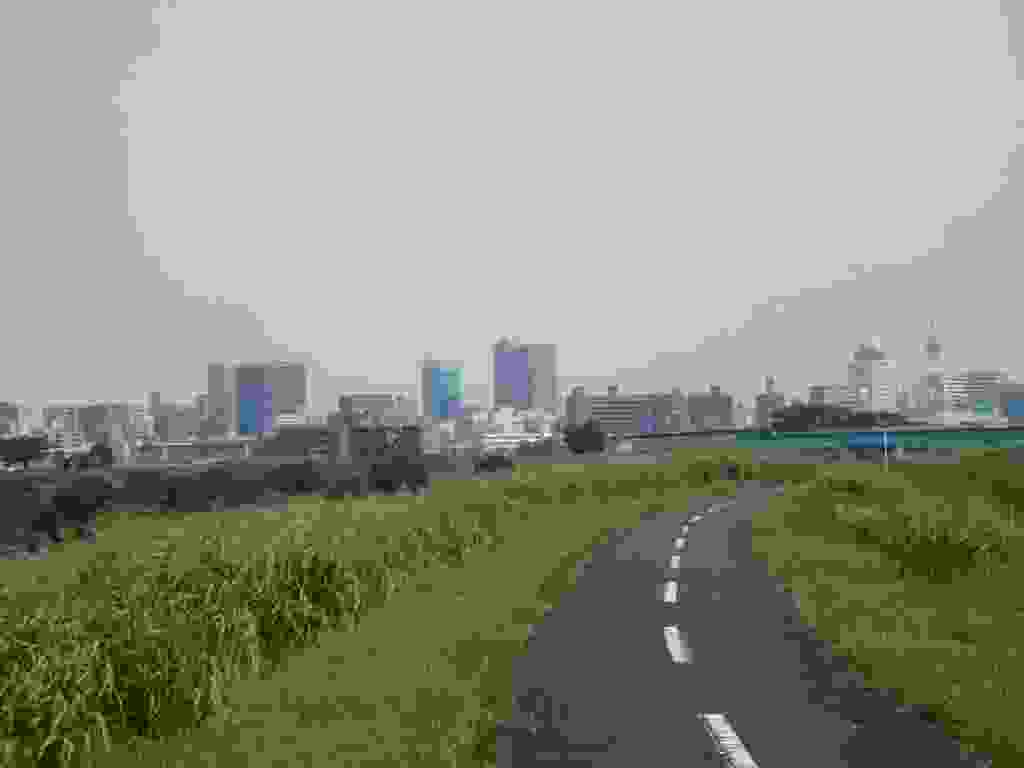
\includegraphics[width=\mywidth]{../wp-content/uploads/2015/08/P7255627-1024x768.jpg} \end{center}
\begin{center} 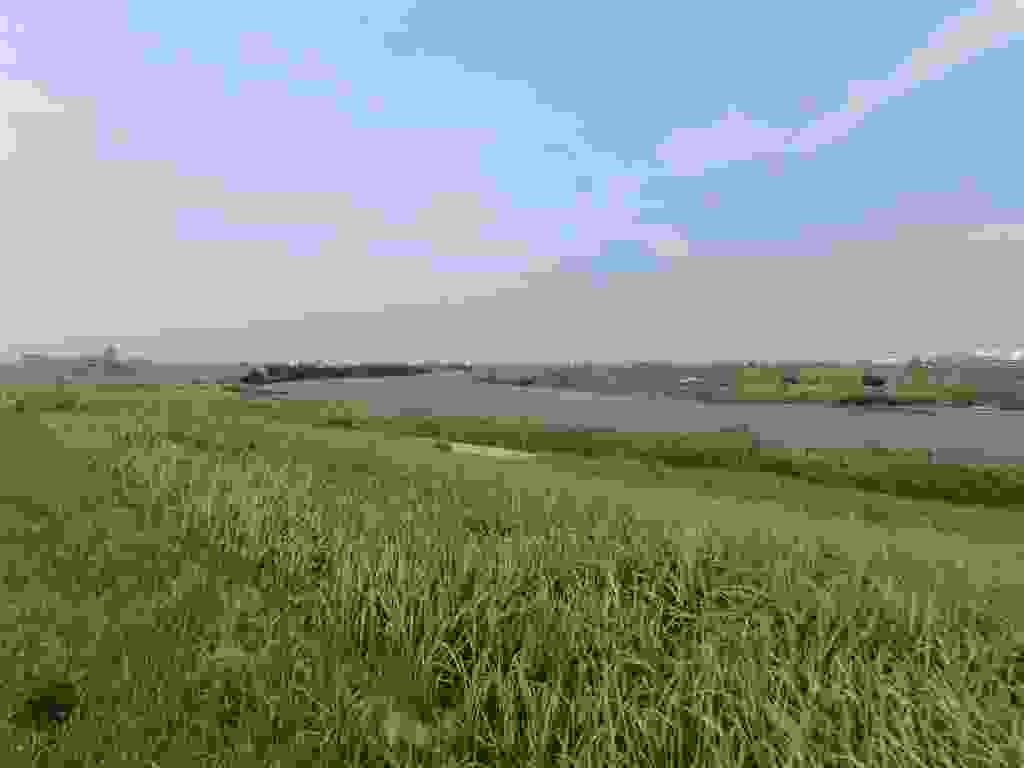
\includegraphics[width=\mywidth]{../wp-content/uploads/2015/08/P7255626-1024x768.jpg} \end{center}
~
\begin{center} 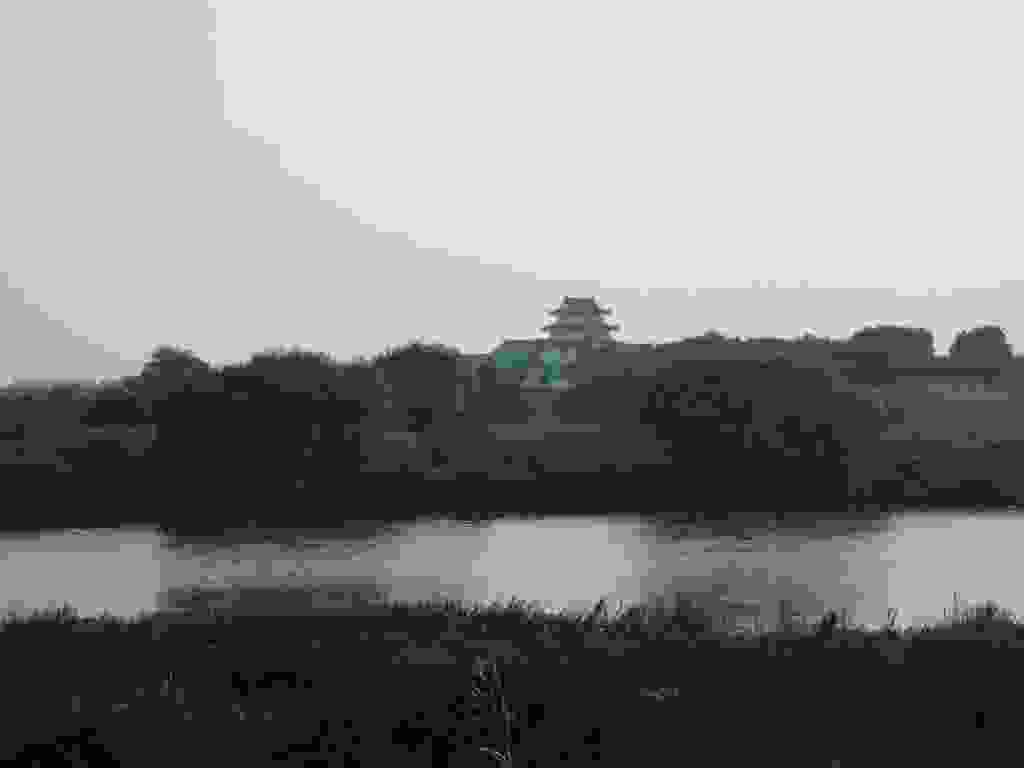
\includegraphics[width=\mywidth]{../wp-content/uploads/2015/08/P7255632-1024x768.jpg} \end{center}
\begin{center} 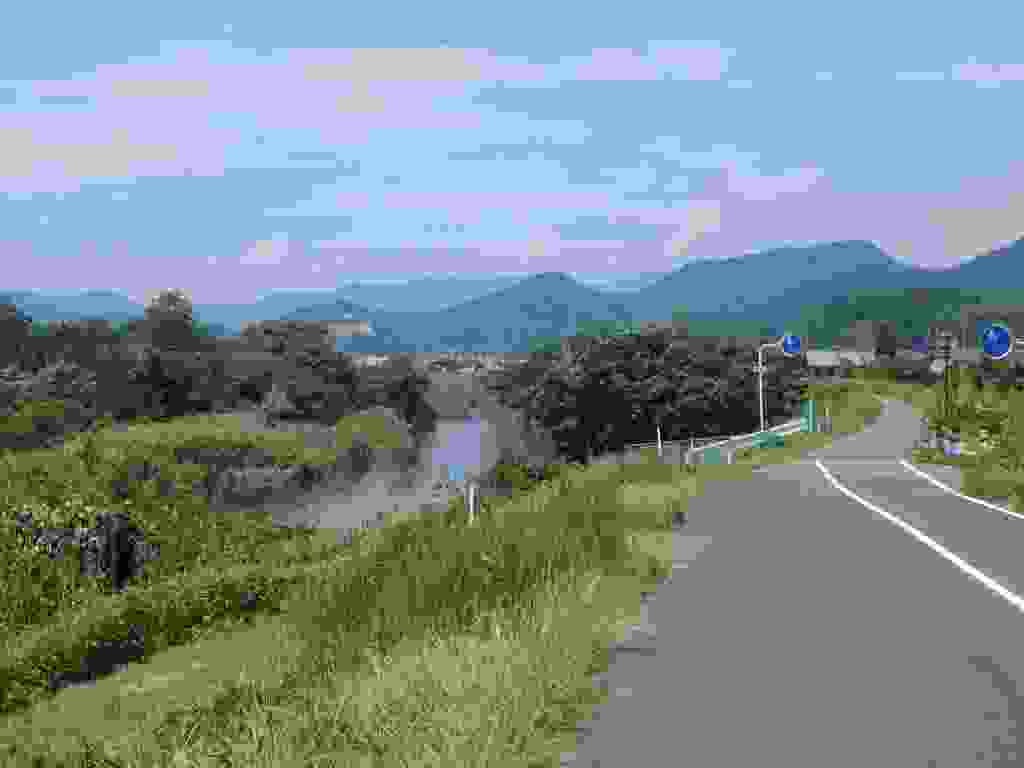
\includegraphics[width=\mywidth]{../wp-content/uploads/2015/08/P7265654-1024x768.jpg} \end{center}

 Le Japon est tellement sûr que je peux camper un peu partout. 
\begin{center} 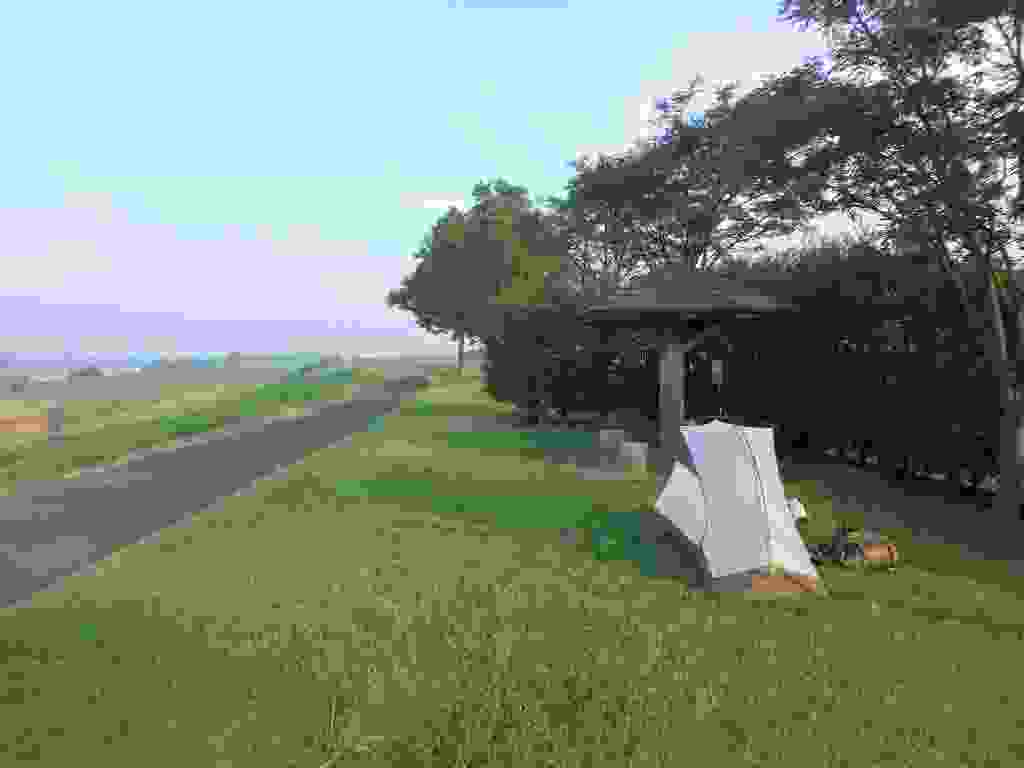
\includegraphics[width=\mywidth]{../wp-content/uploads/2015/08/P7265649-1024x768.jpg} \end{center}
\vspace{-\topsep}
\pagebreak

 Festival dans une ville ou je me suis arreté pour une soirée, avec un concert de jazz.
\begin{center} 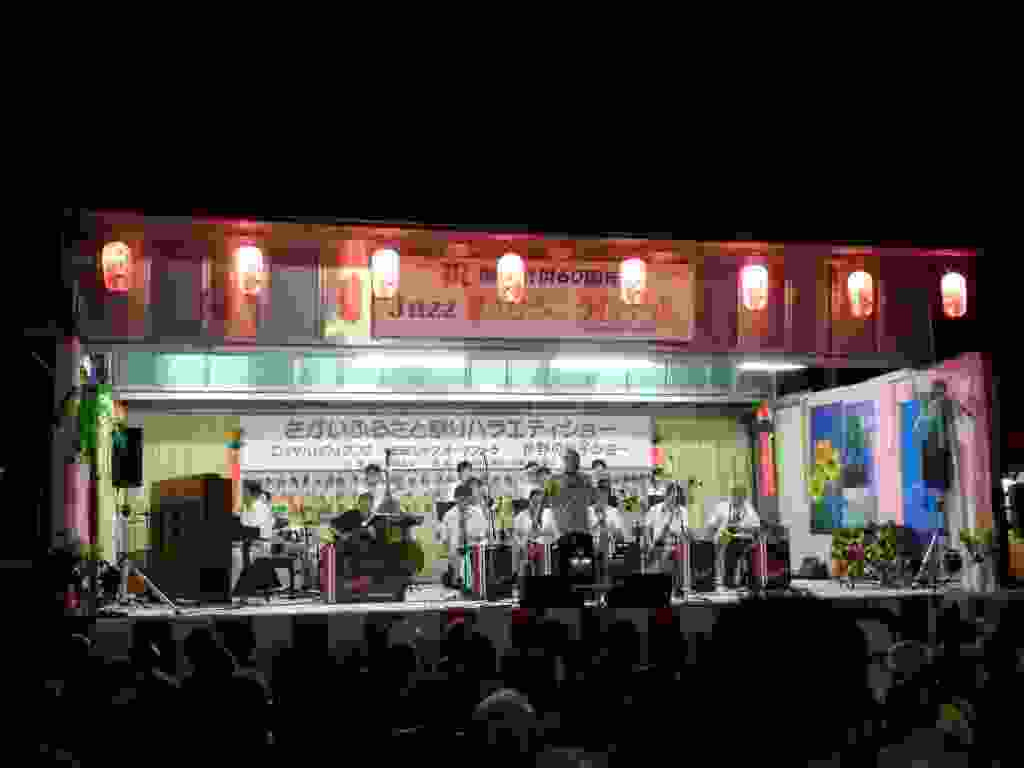
\includegraphics[width=\mywidth]{../wp-content/uploads/2015/08/P7255643-1024x768.jpg} \end{center}

 Et un spectacle de hip hop par des enfants, très fun ! 
\begin{center} 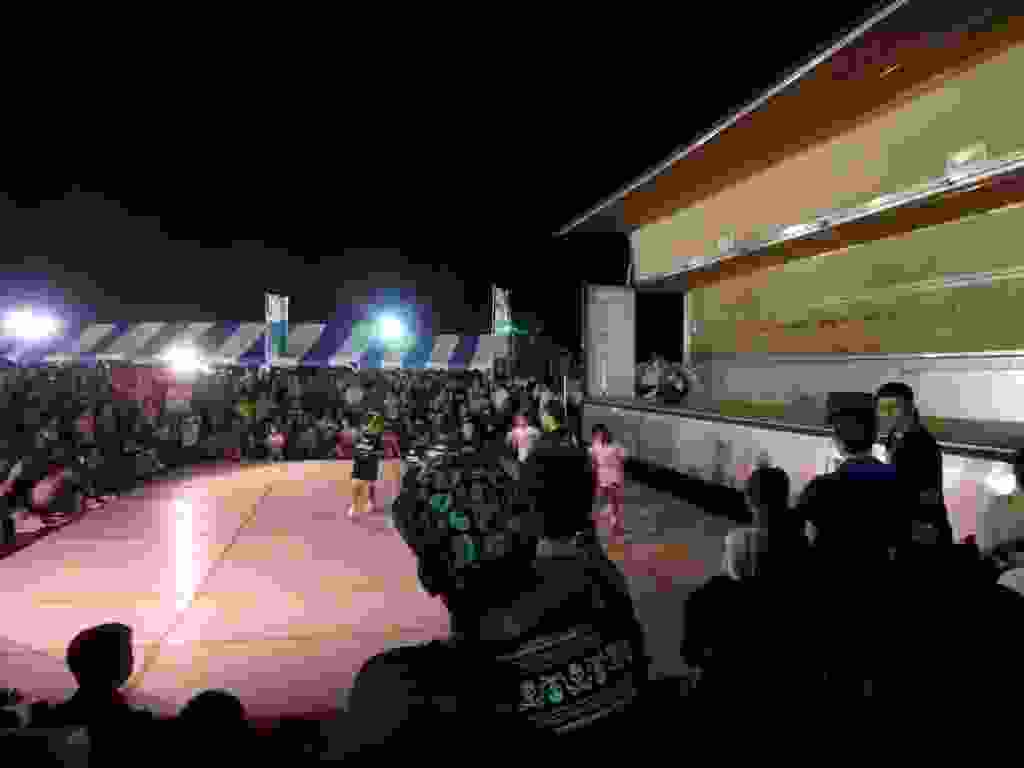
\includegraphics[width=\mywidth]{../wp-content/uploads/2015/08/P7255645-1024x768.jpg} \end{center}
\vspace{-\topsep}
\pagebreak

 La route commence à s'élever, camping au bord d'un lac.\\
\begin{center} 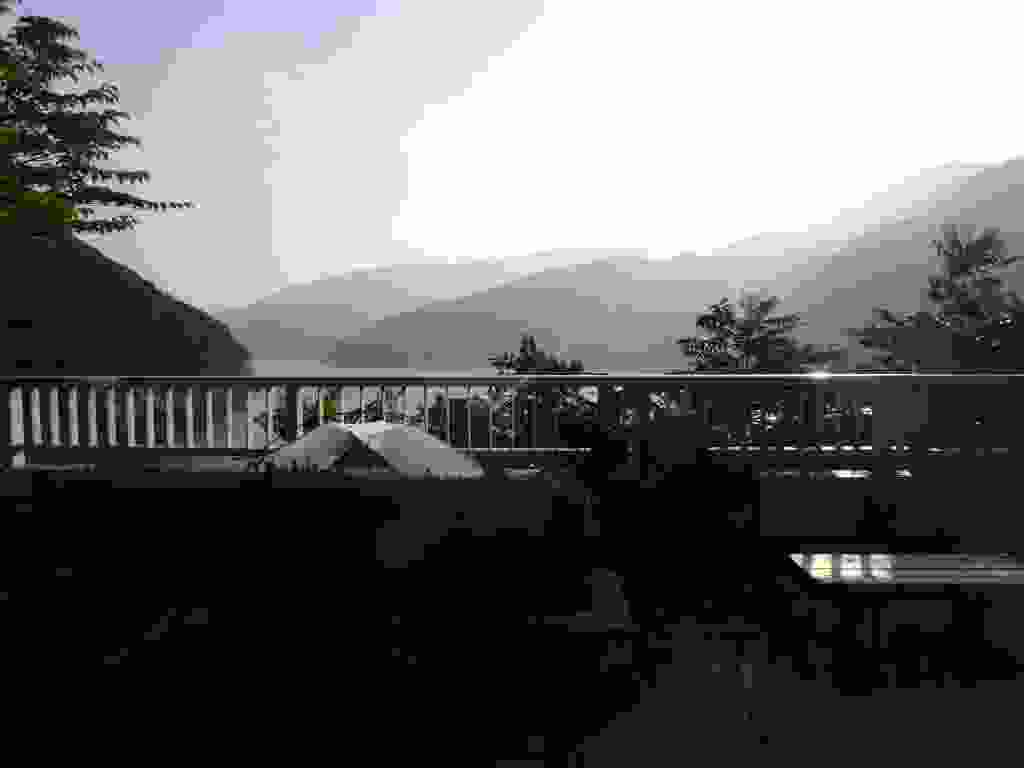
\includegraphics[width=\mywidth]{../wp-content/uploads/2015/08/P7275663-1024x768.jpg} \end{center}
~
\begin{center} 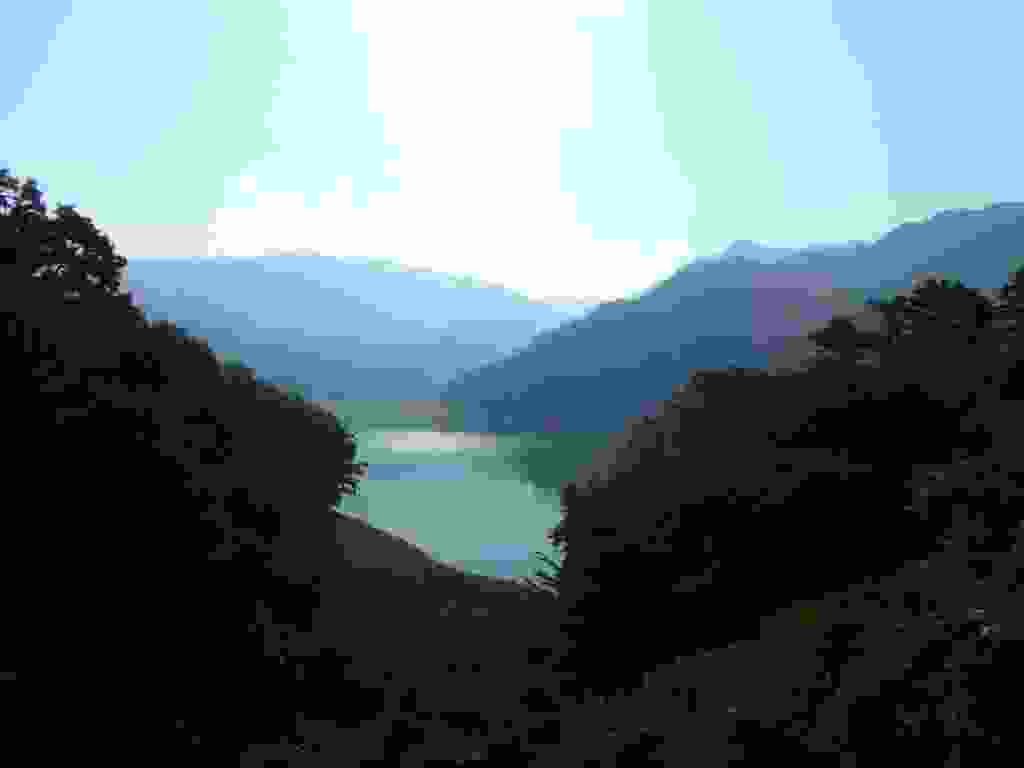
\includegraphics[width=\mywidth]{../wp-content/uploads/2015/08/P7275665-1024x768.jpg} \end{center}
\vspace{-\topsep}
\pagebreak
~
\begin{center} 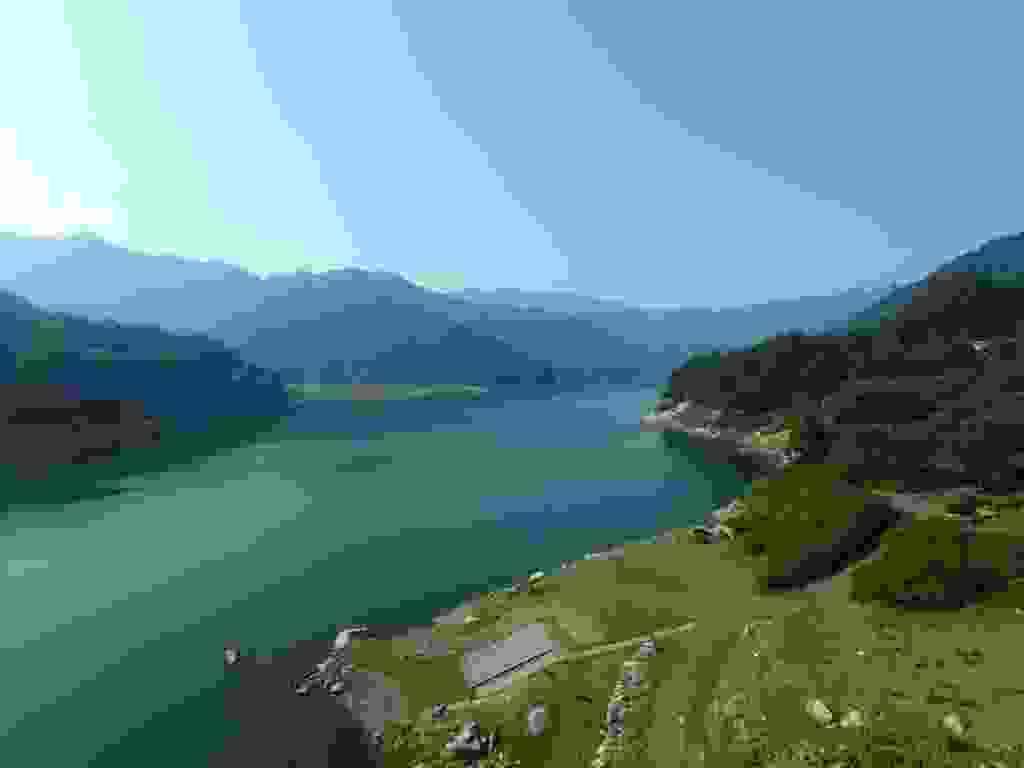
\includegraphics[width=\mywidth]{../wp-content/uploads/2015/08/P7275667-1024x768.jpg} \end{center}
~\\
\begin{center} 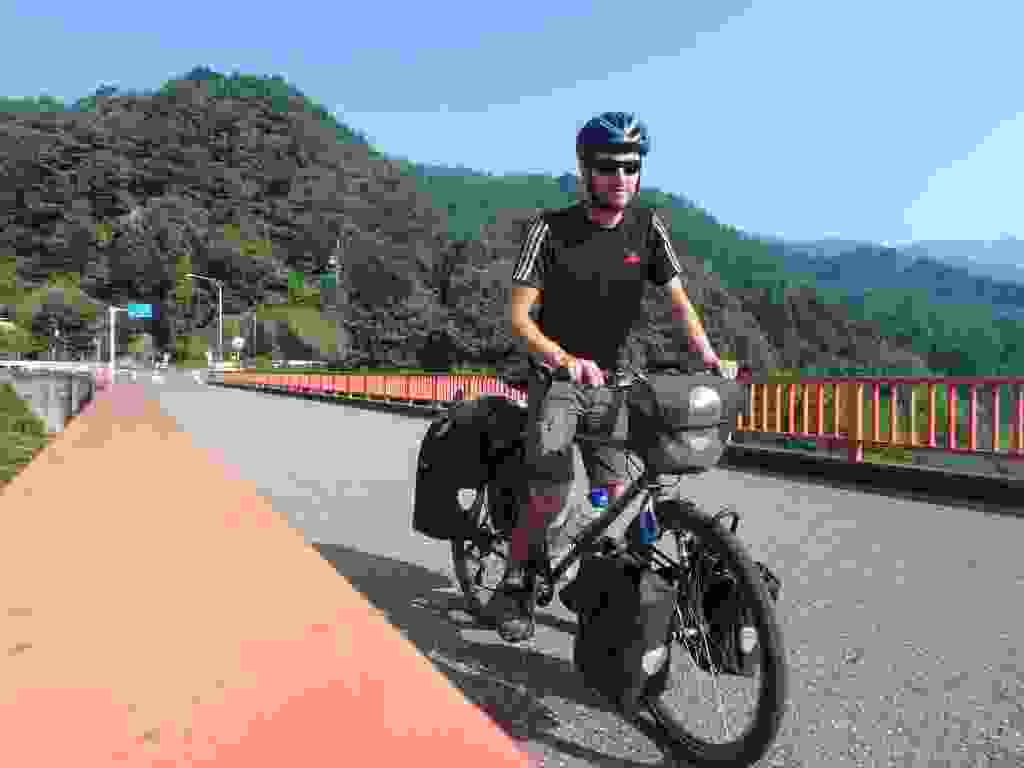
\includegraphics[width=\mywidth]{../wp-content/uploads/2015/08/P7275668-1024x768.jpg} \end{center}
\vspace{-\topsep}
\pagebreak

 Au sommet d'un col je croise des singes.
\begin{center} 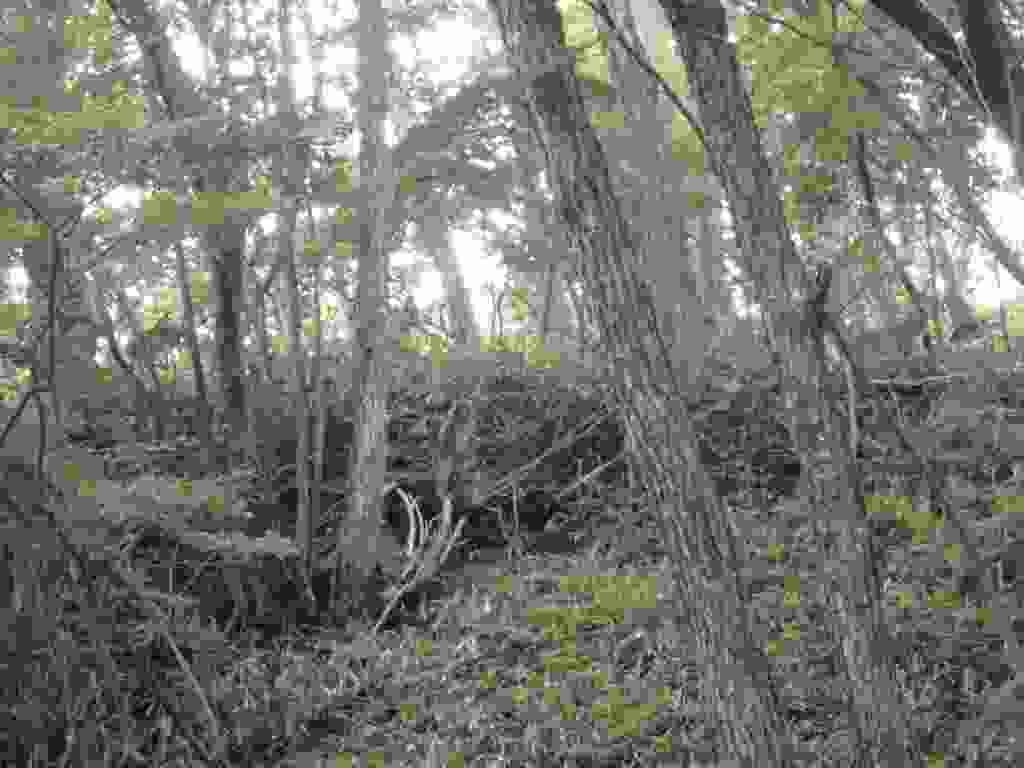
\includegraphics[width=\mywidth]{../wp-content/uploads/2015/08/P7275672-1024x768.jpg} \end{center}

 J'arrive à Nikko, célèbre pour ses temples et shrines inscrits au patrimoine de l'Unesco. 
\begin{center} 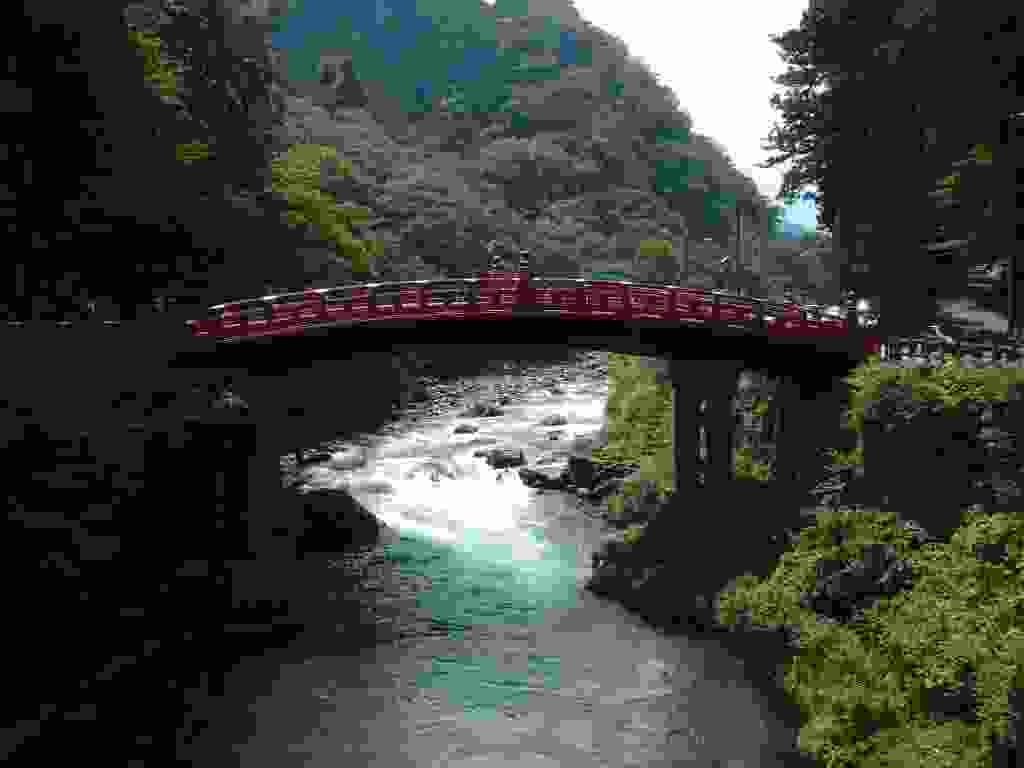
\includegraphics[width=\mywidth]{../wp-content/uploads/2015/08/P7275678-1024x768.jpg} \end{center}
\vspace{-\topsep}
\pagebreak
~
\begin{center} 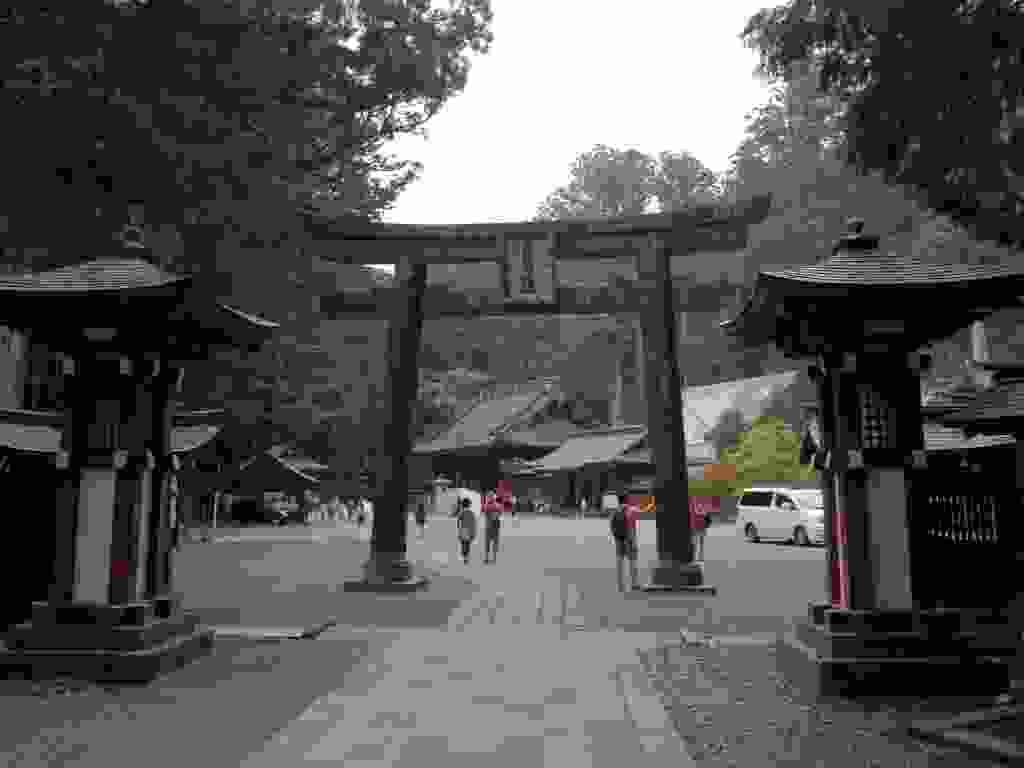
\includegraphics[width=\mywidth]{../wp-content/uploads/2015/08/P7285733-1024x768.jpg} \end{center}

  Beaucoup de groupes d'enfants japonais visitent Nikko, des jeunes viennent me poser des questions pour s'exercer en anglais. 
\begin{center} 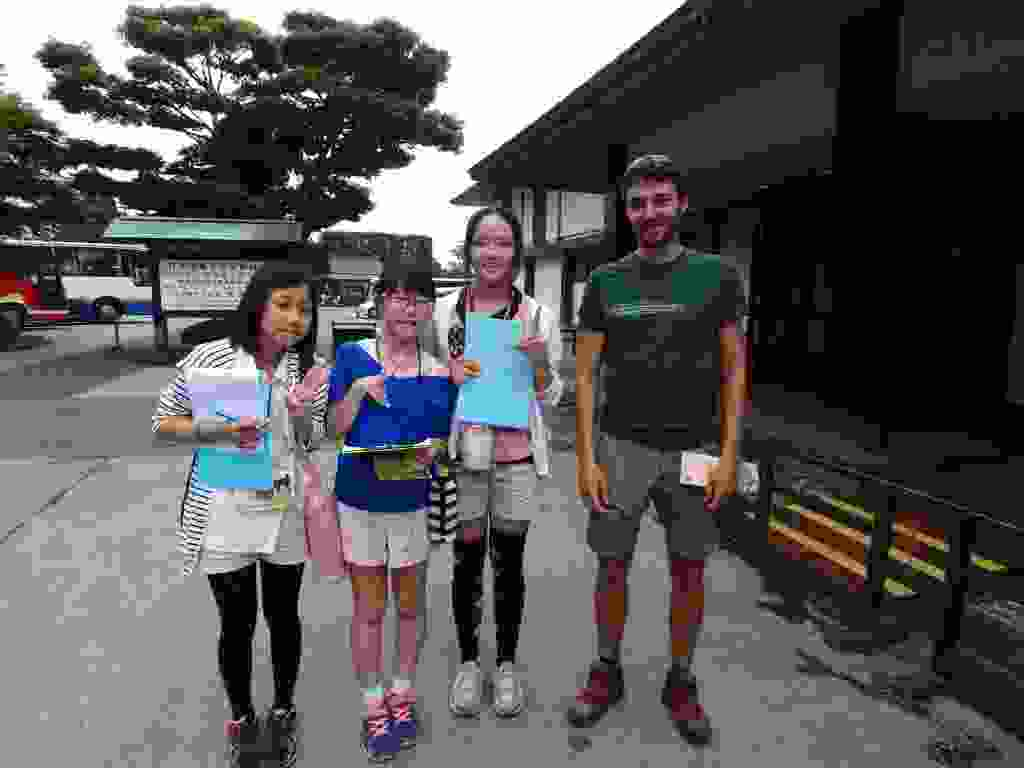
\includegraphics[width=\mywidth]{../wp-content/uploads/2015/08/P7285692-1024x768.jpg} \end{center}
\vspace{-\topsep}
\pagebreak

 Le temple de Toshogu avec le mausolée du Shogun Tokugawa Ieyasu. 
\begin{center} 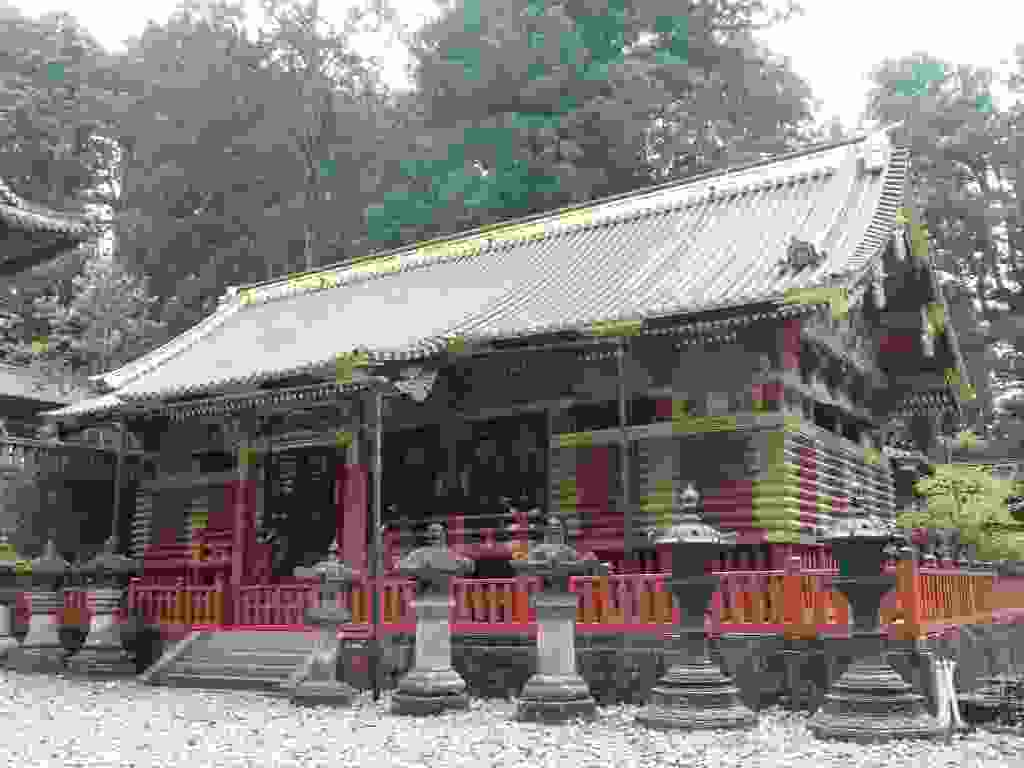
\includegraphics[width=\mywidth]{../wp-content/uploads/2015/08/P7285706-1024x768.jpg} \end{center}
~\\
\begin{center} 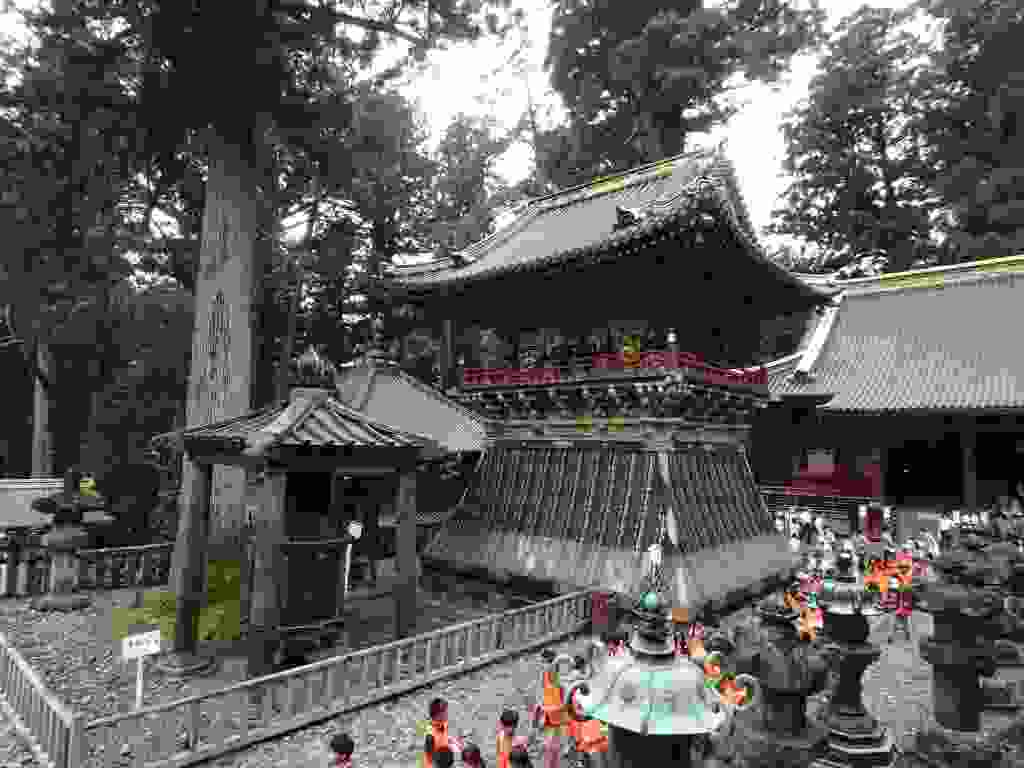
\includegraphics[width=\mywidth]{../wp-content/uploads/2015/08/P7285727-1024x768.jpg} \end{center}
\vspace{-\topsep}
\pagebreak
~\\
\begin{center} 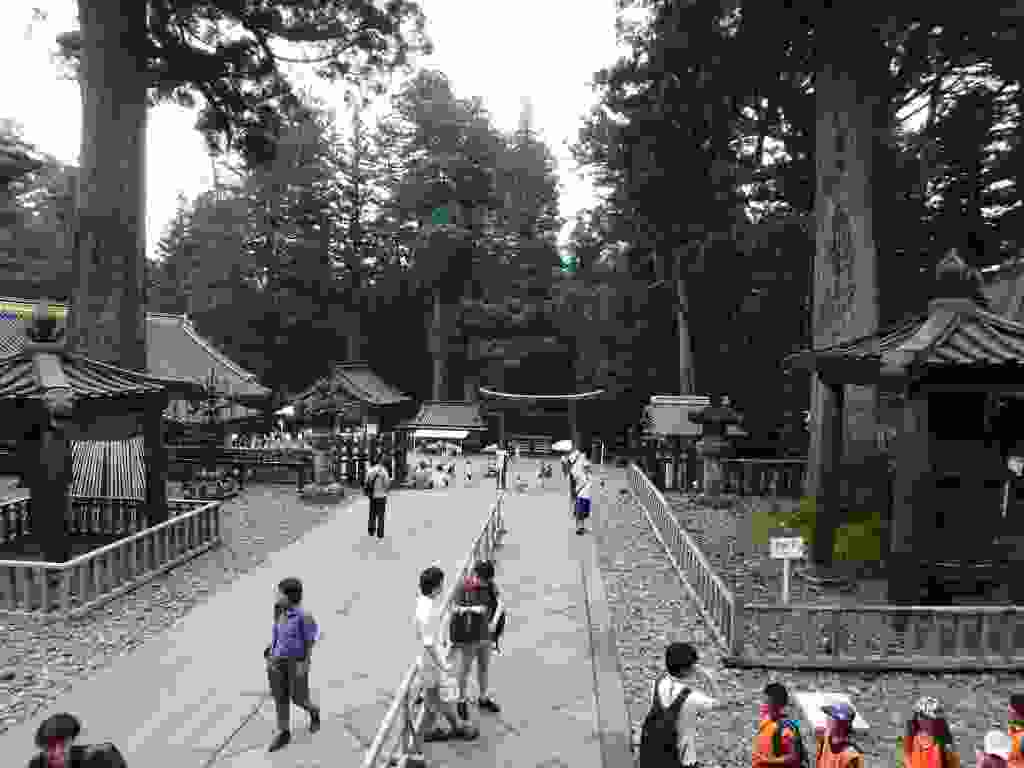
\includegraphics[width=\mywidth]{../wp-content/uploads/2015/08/P7285726-1024x768.jpg} \end{center}
~
\begin{center} 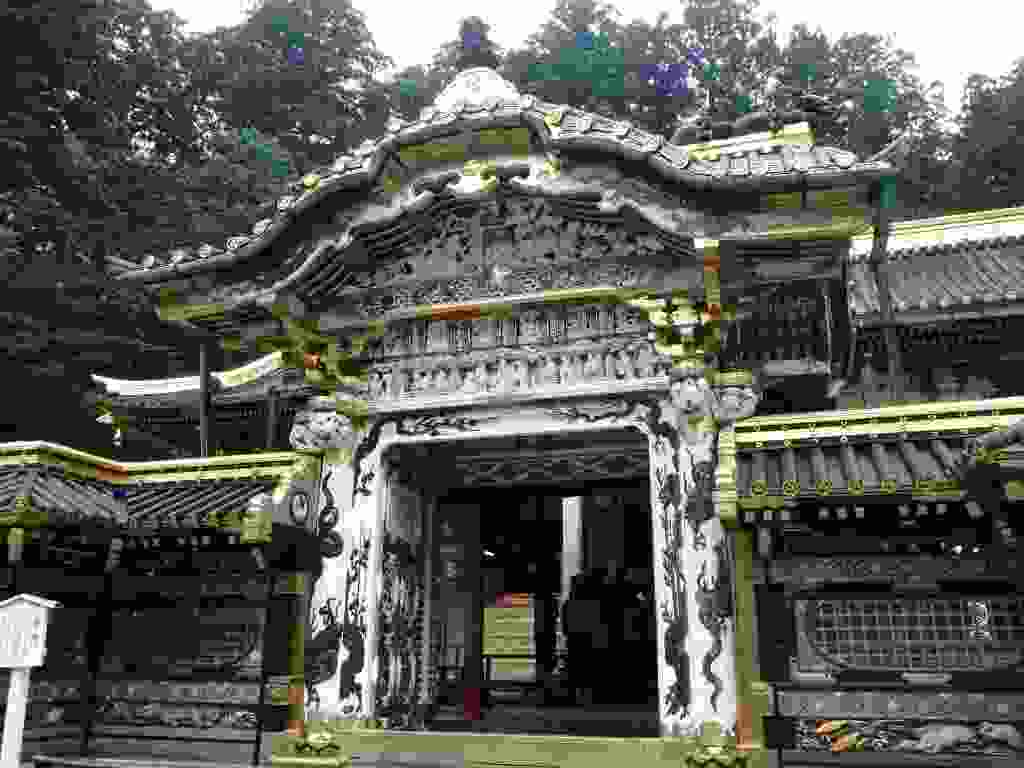
\includegraphics[width=\mywidth]{../wp-content/uploads/2015/08/P7285724-1024x768.jpg} \end{center}
\vspace{-\topsep}
\pagebreak

 Représentation des 3 singes sages : \og ne rien voir, ne rien entendre, ne rien dire \fg.
\begin{center} 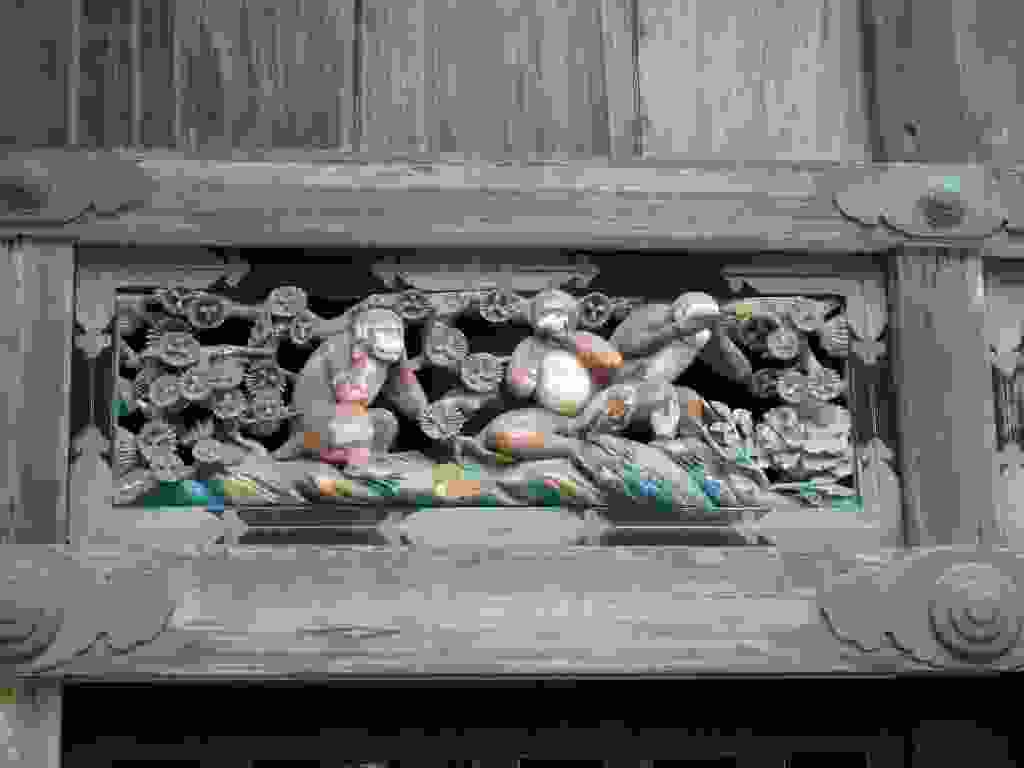
\includegraphics[width=\mywidth]{../wp-content/uploads/2015/08/P7285703-1024x768.jpg} \end{center}

 Le shrine de Taiyuin.
\begin{center} 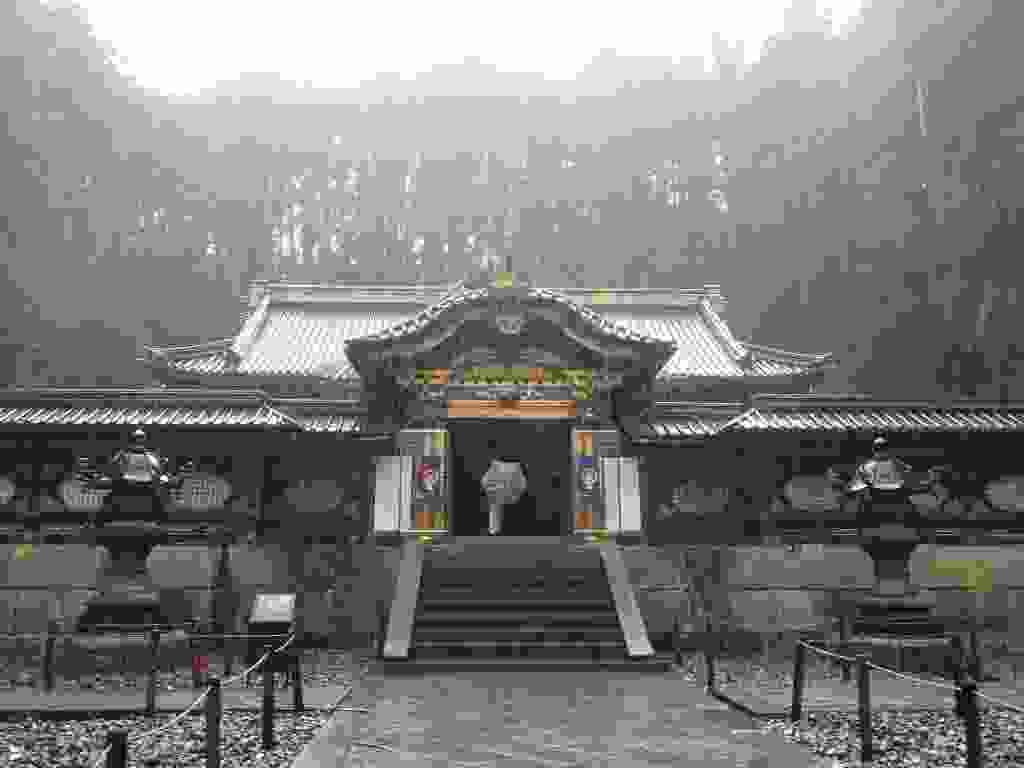
\includegraphics[width=\mywidth]{../wp-content/uploads/2015/08/P7285745-1024x768.jpg} \end{center}
\vspace{-\topsep}
\pagebreak

 Un chemin dans la forêt permet d'accéder à un petit shrine.
\begin{center} 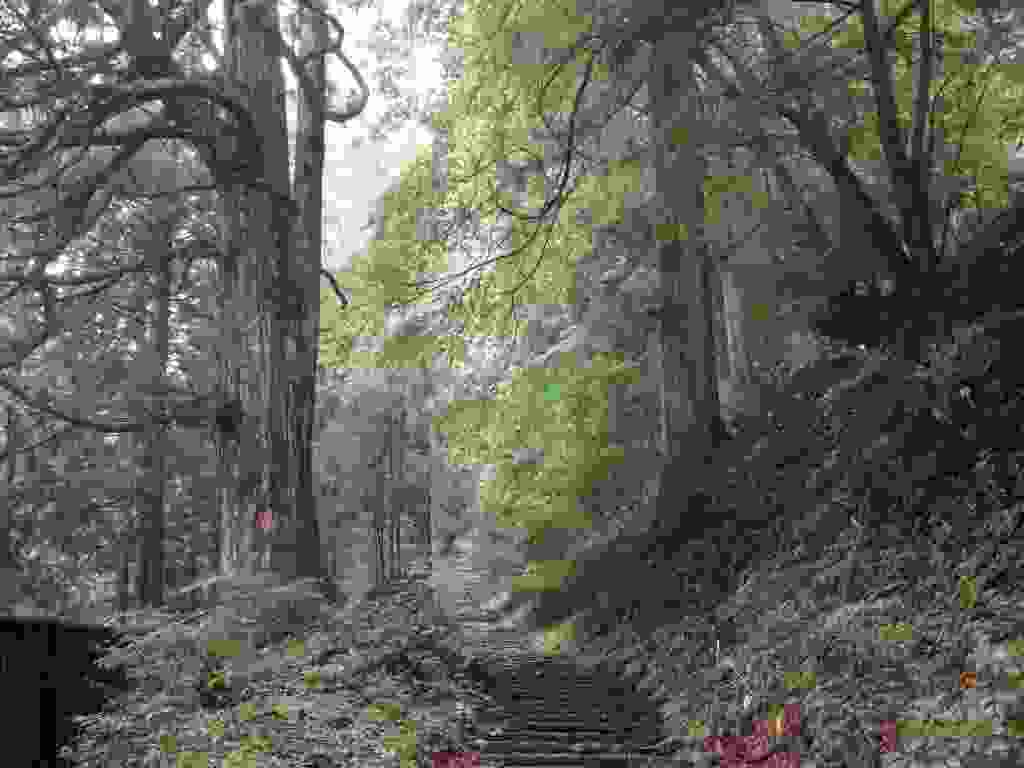
\includegraphics[width=\mywidth]{../wp-content/uploads/2015/08/P7285754-1024x768.jpg} \end{center}
\begin{center} 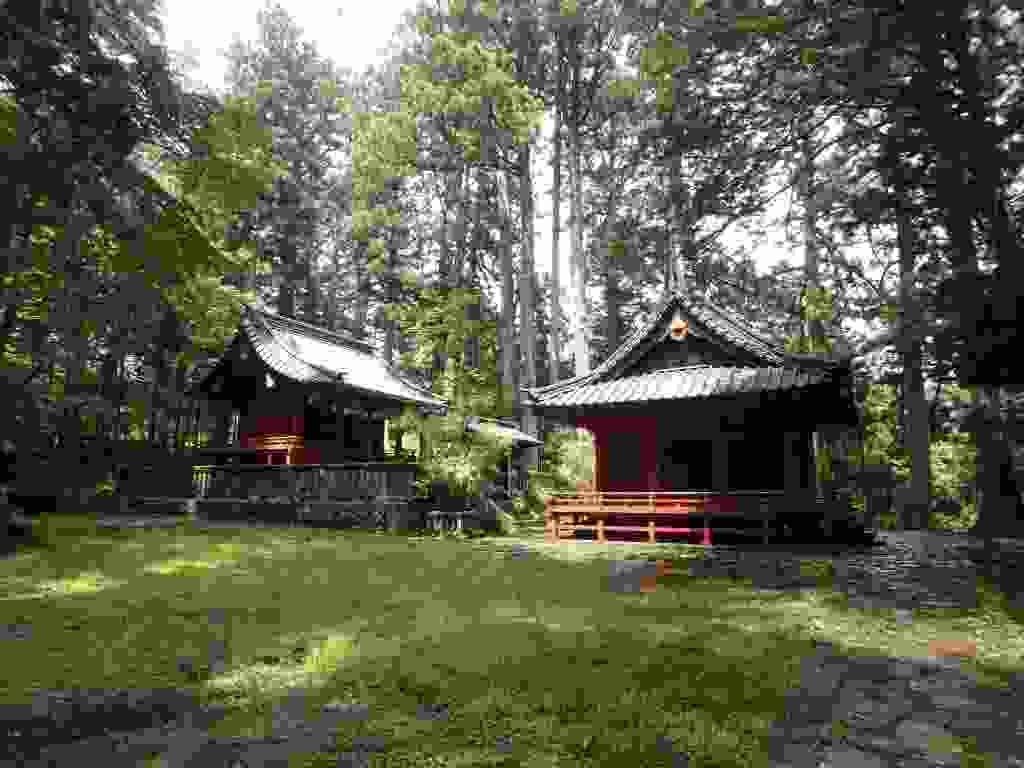
\includegraphics[width=\mywidth]{../wp-content/uploads/2015/08/P7285760-1024x768.jpg} \end{center}
\vspace{-\topsep}
\vspace{-3.25mm}
\pagebreak

 Un alignement impressionnant de Jizo, des protecteurs.
\begin{center} 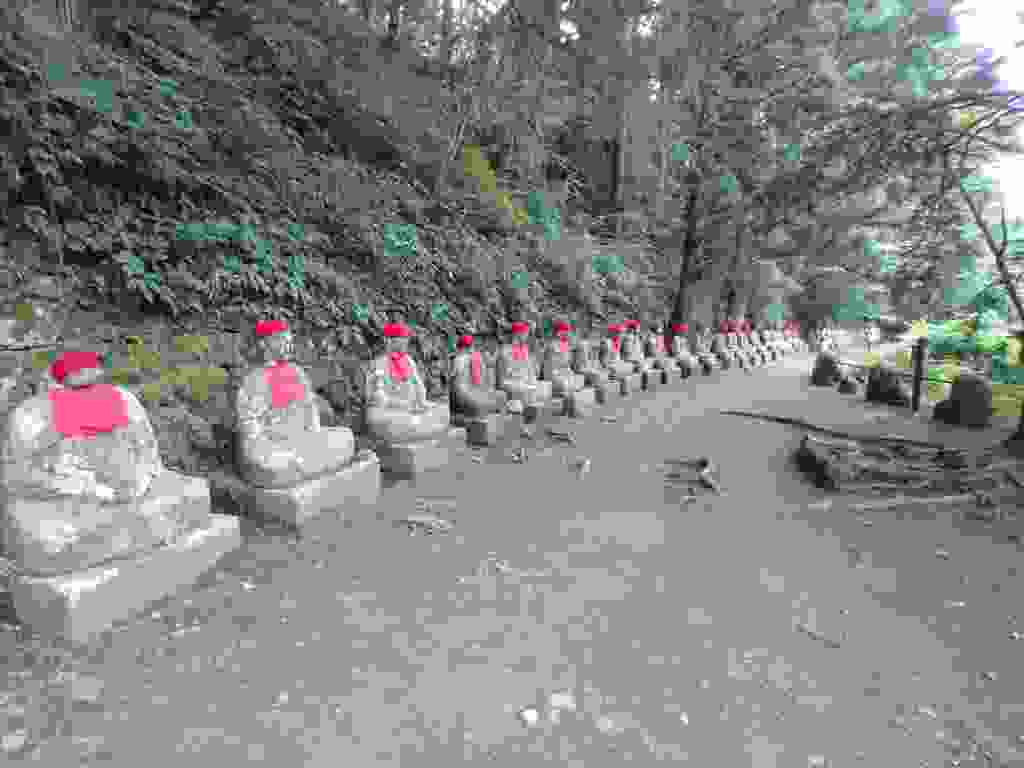
\includegraphics[width=\mywidth]{../wp-content/uploads/2015/08/P7275684-1024x768.jpg} \end{center}
\begin{center} 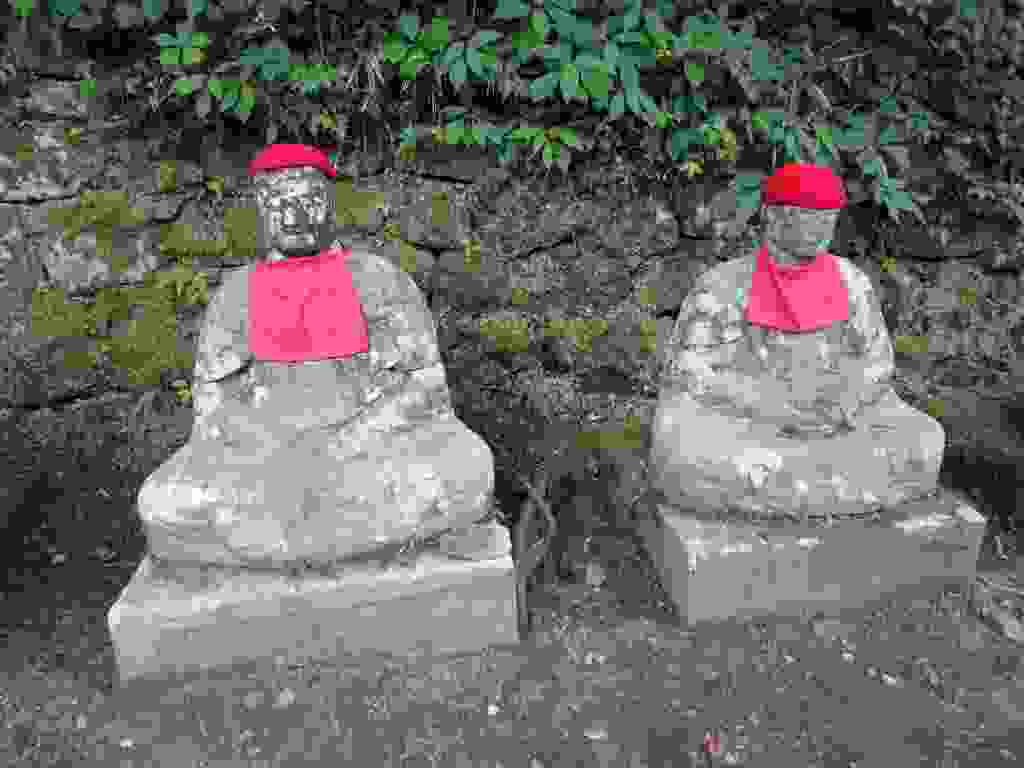
\includegraphics[width=\mywidth]{../wp-content/uploads/2015/08/P7275685-1024x768.jpg} \end{center}
\vspace{-\topsep}
\vspace{-3.25mm}
\pagebreak

 Je repars vers le parc national de Nikko.
\begin{center} 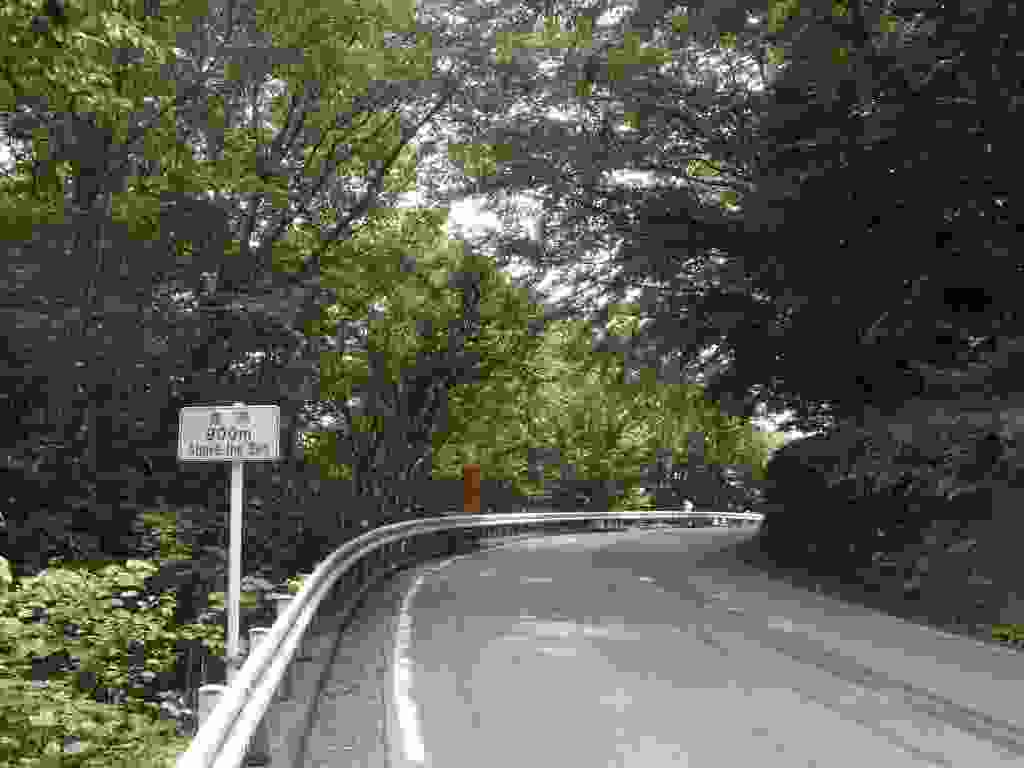
\includegraphics[width=\mywidth]{../wp-content/uploads/2015/08/P7295772-1024x768.jpg} \end{center}
~
\begin{center} 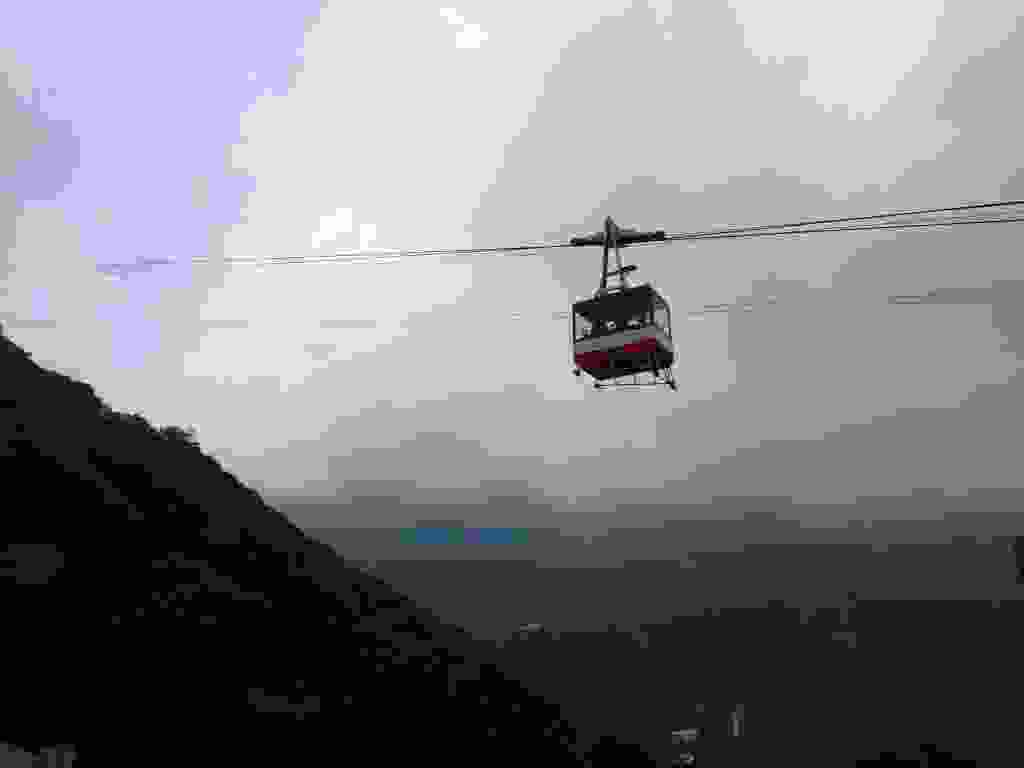
\includegraphics[width=\mywidth]{../wp-content/uploads/2015/08/P7295774-1024x768.jpg} \end{center}
\vspace{-\topsep}
\pagebreak

 La cascade de Kegon.
\begin{center} 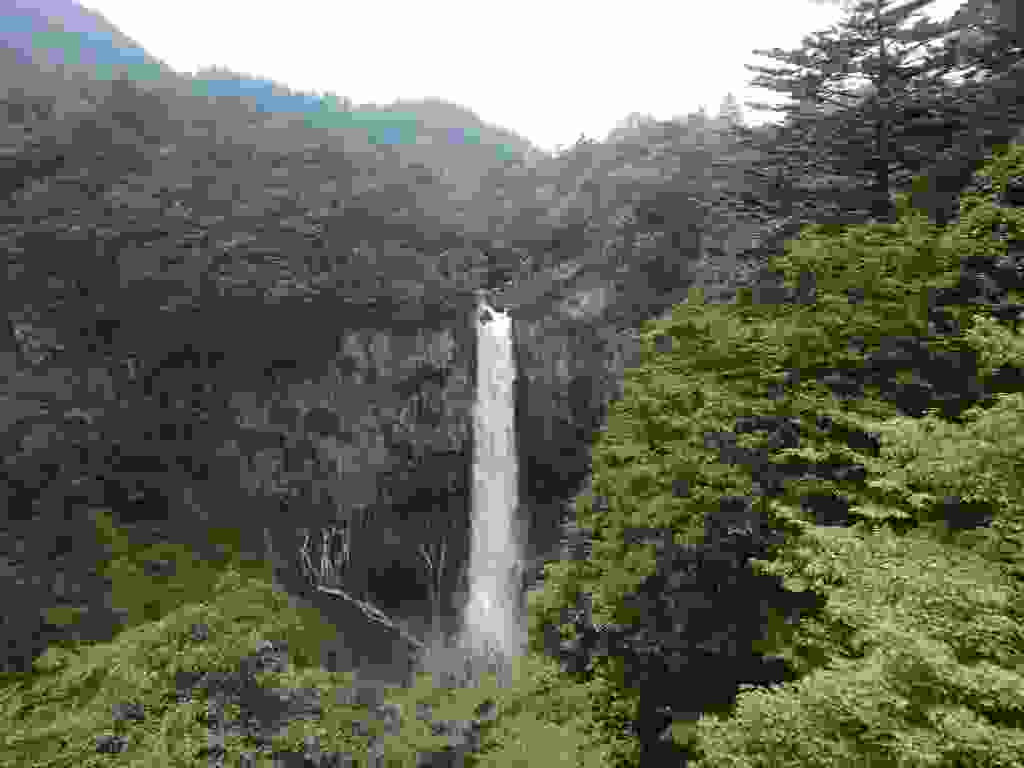
\includegraphics[width=\mywidth]{../wp-content/uploads/2015/08/P7295778-1024x768.jpg} \end{center}

 Balade pour voir le lac Chūzenji, avec un temps pas idéal. 
\begin{center} 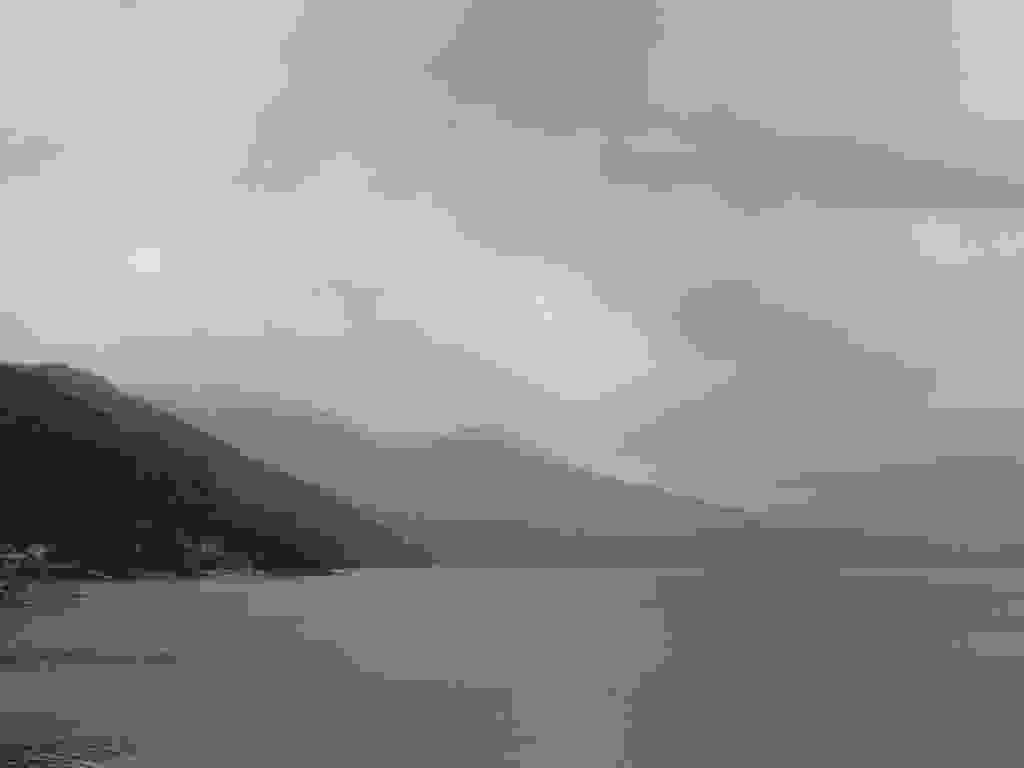
\includegraphics[width=\mywidth]{../wp-content/uploads/2015/08/P7295782-1024x768.jpg} \end{center}
\begin{center} 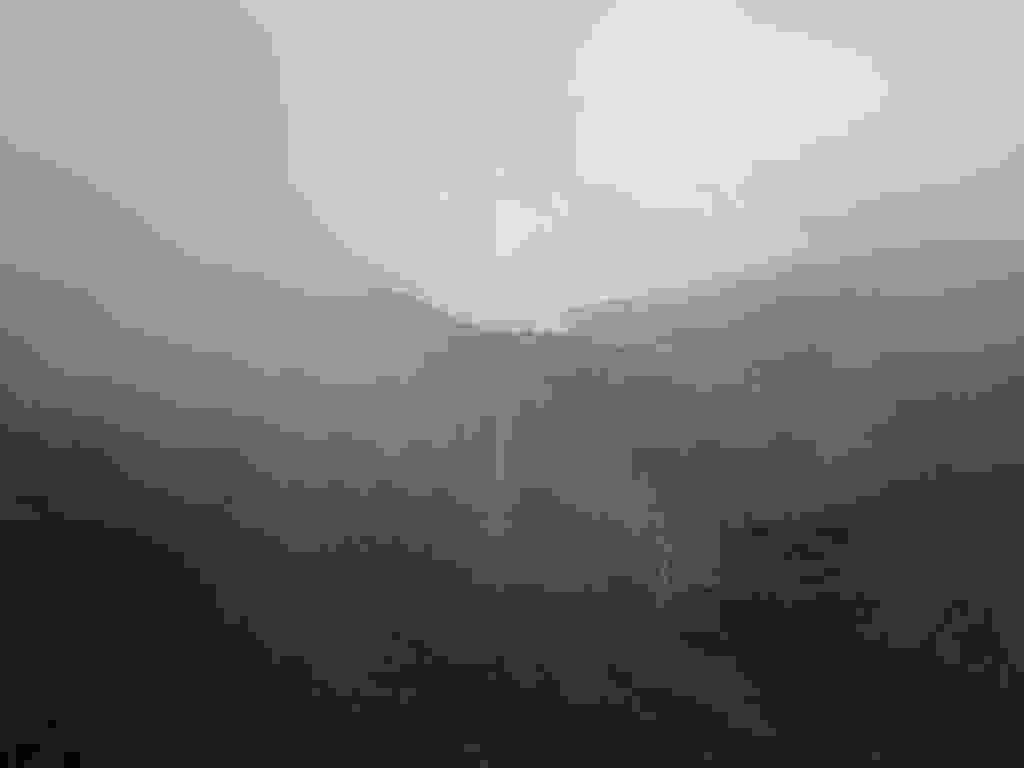
\includegraphics[width=\mywidth]{../wp-content/uploads/2015/08/P7295791-1024x768.jpg} \end{center}

 Je continue la montée jusqu'à la cascade et au lac de Yumoto. 
\begin{center} 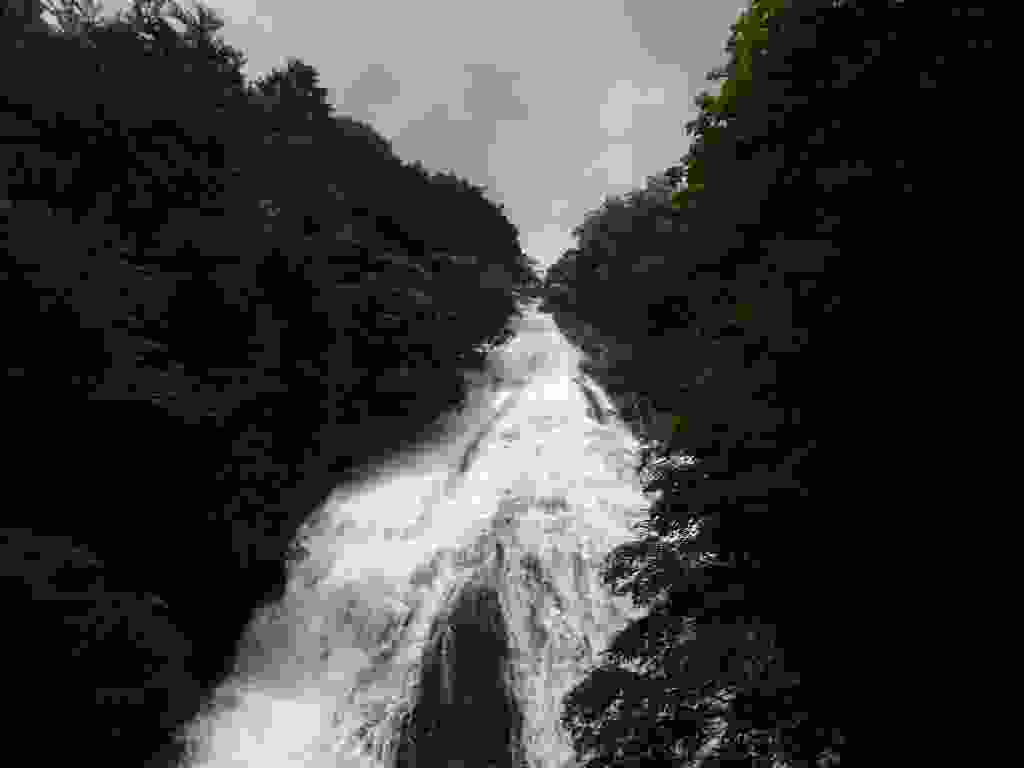
\includegraphics[width=\mywidth]{../wp-content/uploads/2015/08/P7305824-1024x768.jpg} \end{center}
\begin{center} 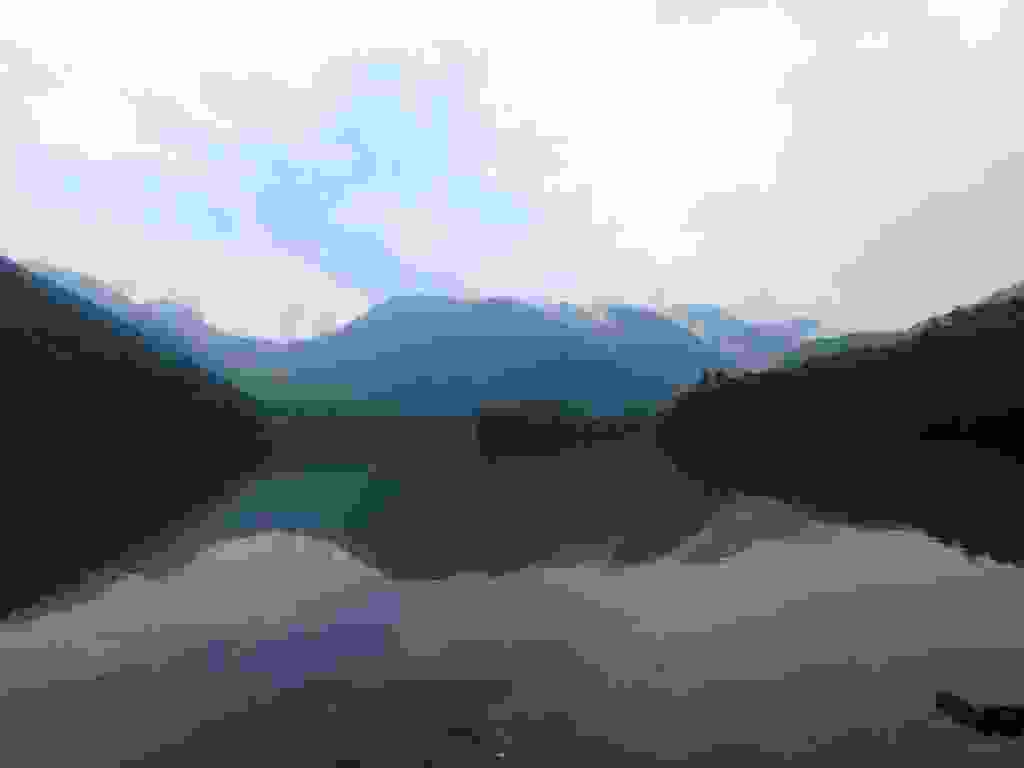
\includegraphics[width=\mywidth]{../wp-content/uploads/2015/08/P7305825-1024x768.jpg} \end{center}
~
\begin{center} 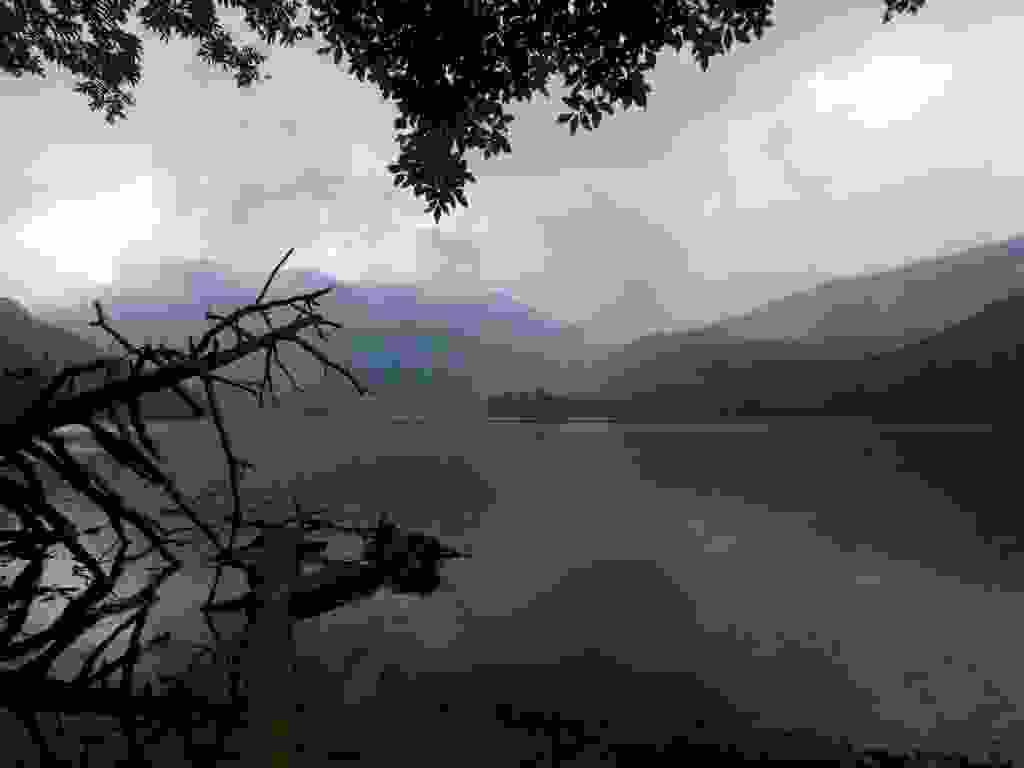
\includegraphics[width=\mywidth]{../wp-content/uploads/2015/08/P7305820-1024x768.jpg} \end{center}
\vspace{-\topsep}
\pagebreak

 Yumoto est aussi connu pour ses onsen, ou sources chaudes.
\begin{center} 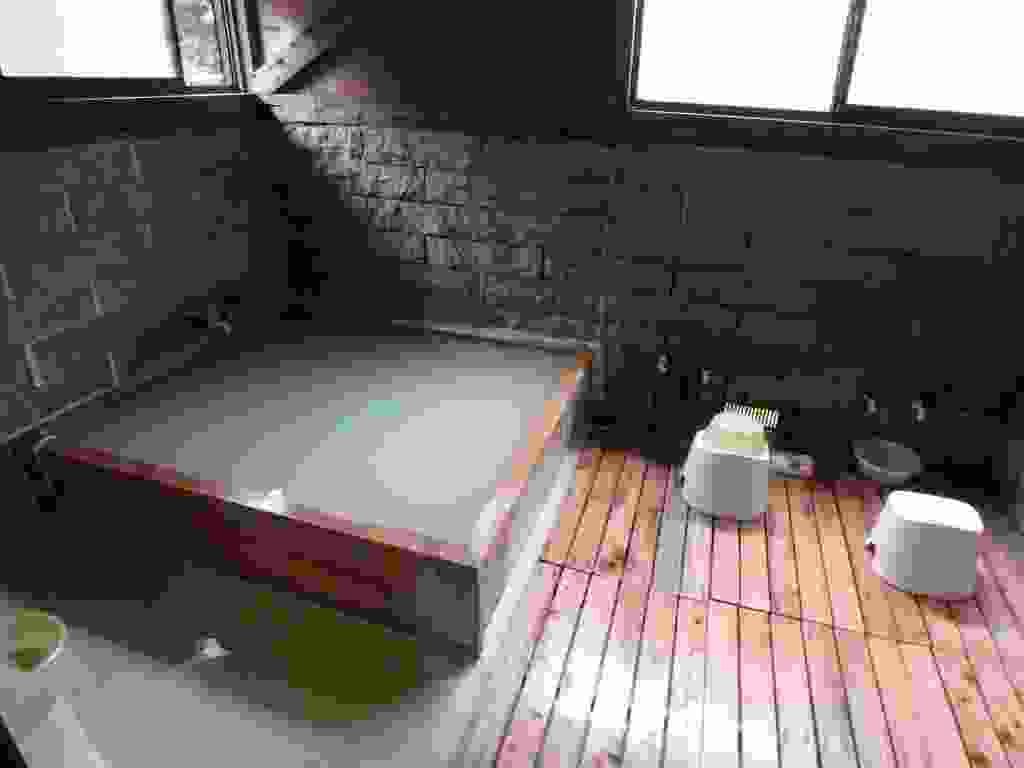
\includegraphics[width=\mywidth]{../wp-content/uploads/2015/08/P7305829-1024x768.jpg} \end{center}

 Je passe ensuite le col de Konsei à plus de 2000m.
\begin{center} 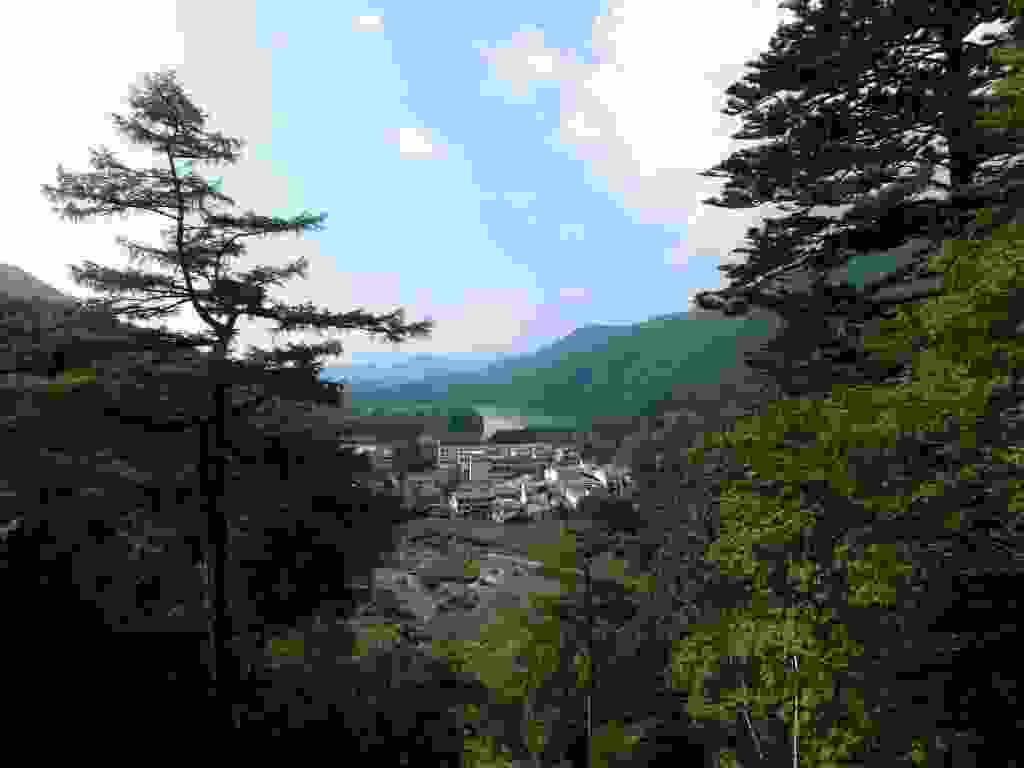
\includegraphics[width=\mywidth]{../wp-content/uploads/2015/08/P7315831-1024x768.jpg} \end{center}
\vspace{-\topsep}
\pagebreak
~
\begin{center} 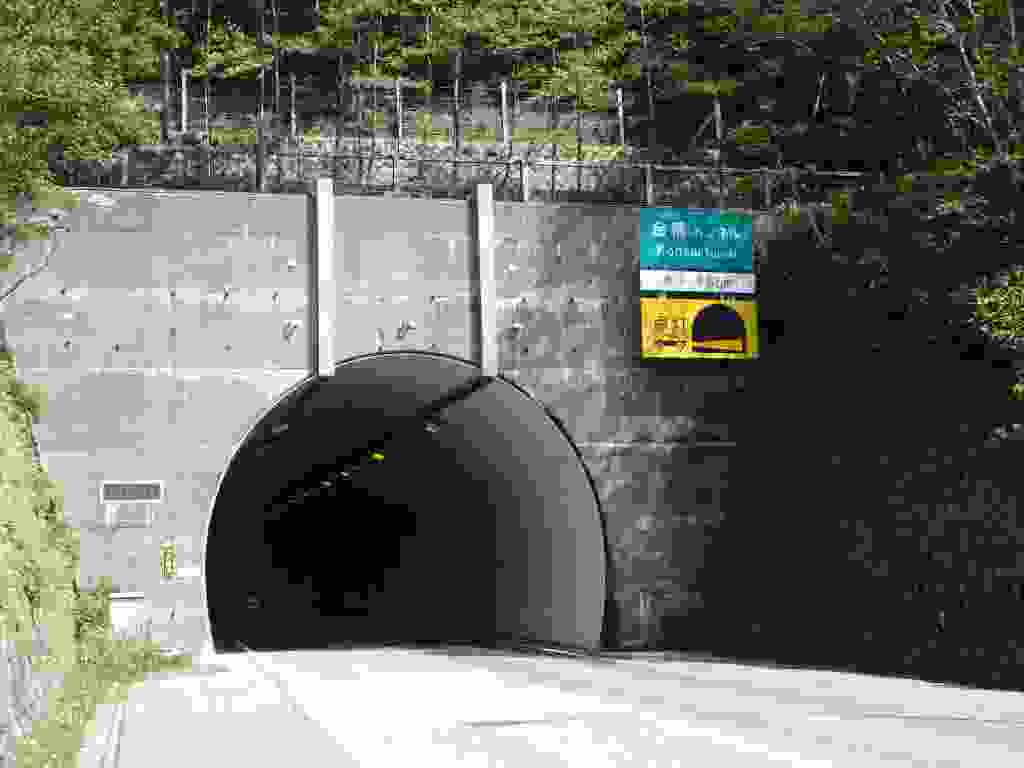
\includegraphics[width=\mywidth]{../wp-content/uploads/2015/08/P7315837-1024x768.jpg} \end{center}
~
\begin{center} 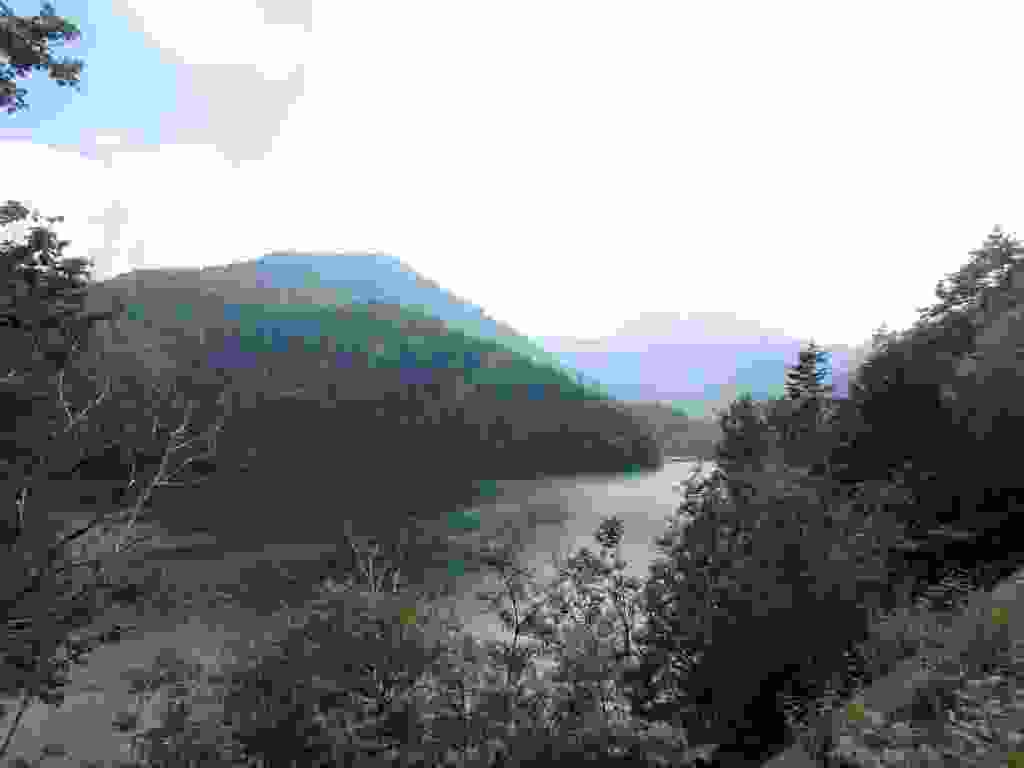
\includegraphics[width=\mywidth]{../wp-content/uploads/2015/08/P7315838-1024x768.jpg} \end{center}
\vspace{-\topsep}
\pagebreak

 Je croise une station de ski, l'envie me prend de faire quelques descentes. 
\begin{center} 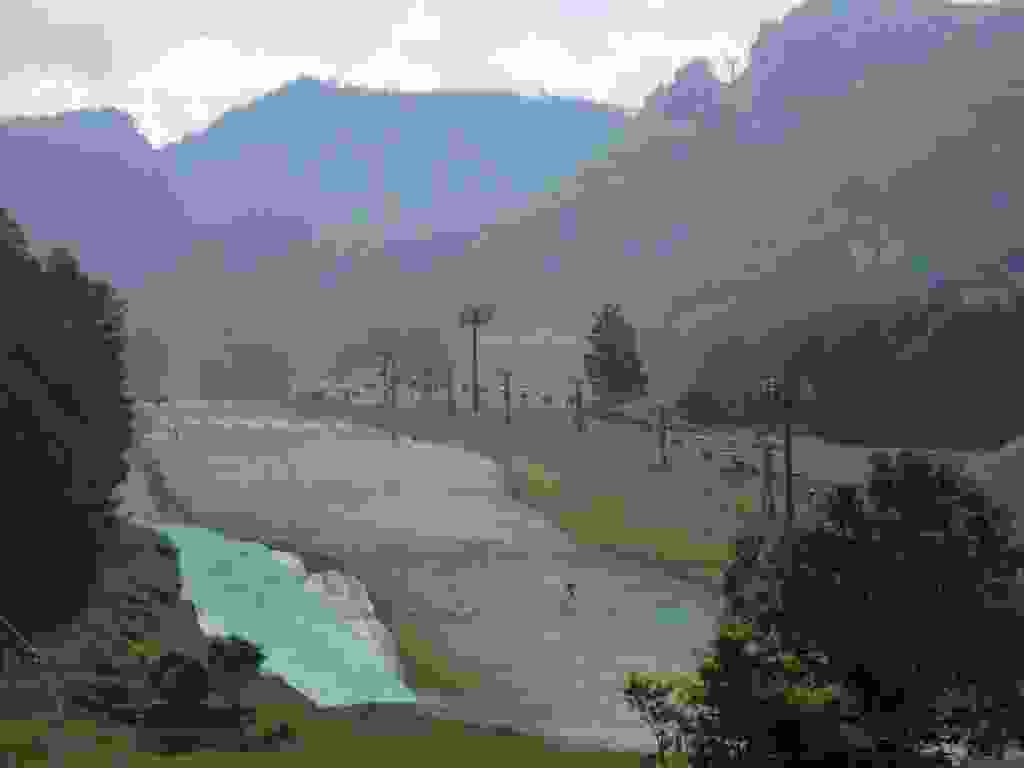
\includegraphics[width=\mywidth]{../wp-content/uploads/2015/08/P7315840-1024x768.jpg} \end{center}
\begin{center} 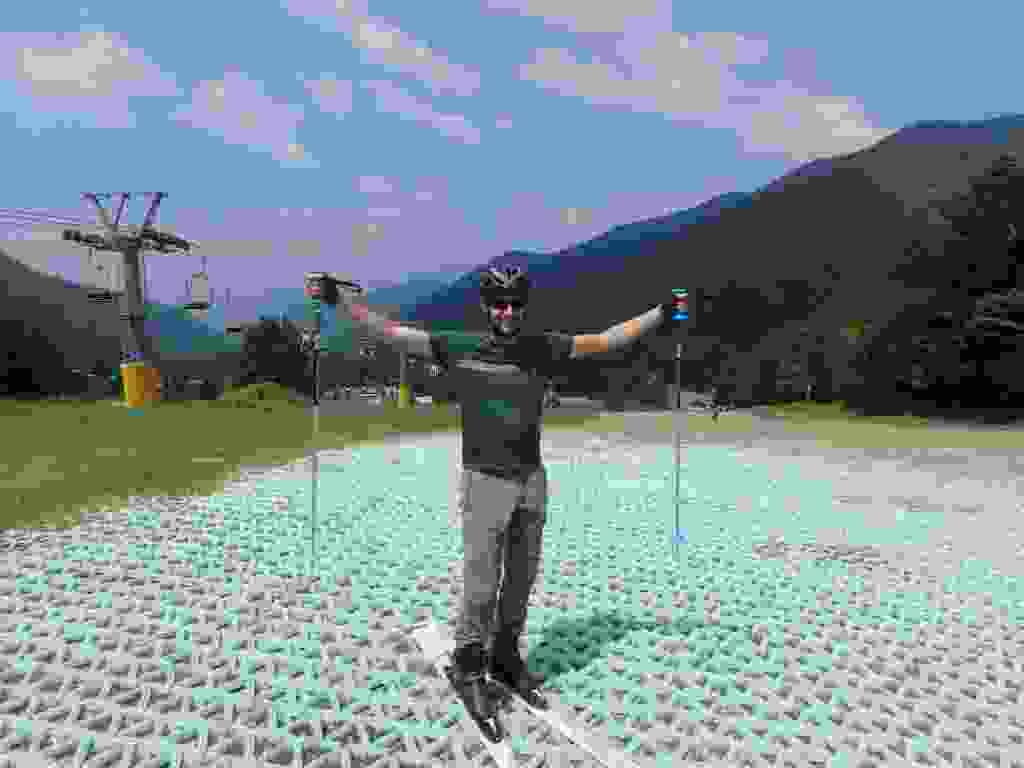
\includegraphics[width=\mywidth]{../wp-content/uploads/2015/08/P7315847-1024x768.jpg} \end{center}
\vspace{-\topsep}
\vspace{-2.75mm}
\pagebreak

 J'emprunte la route romantique japonaise qui ressemble à la route allemande du même nom. 
\begin{center} 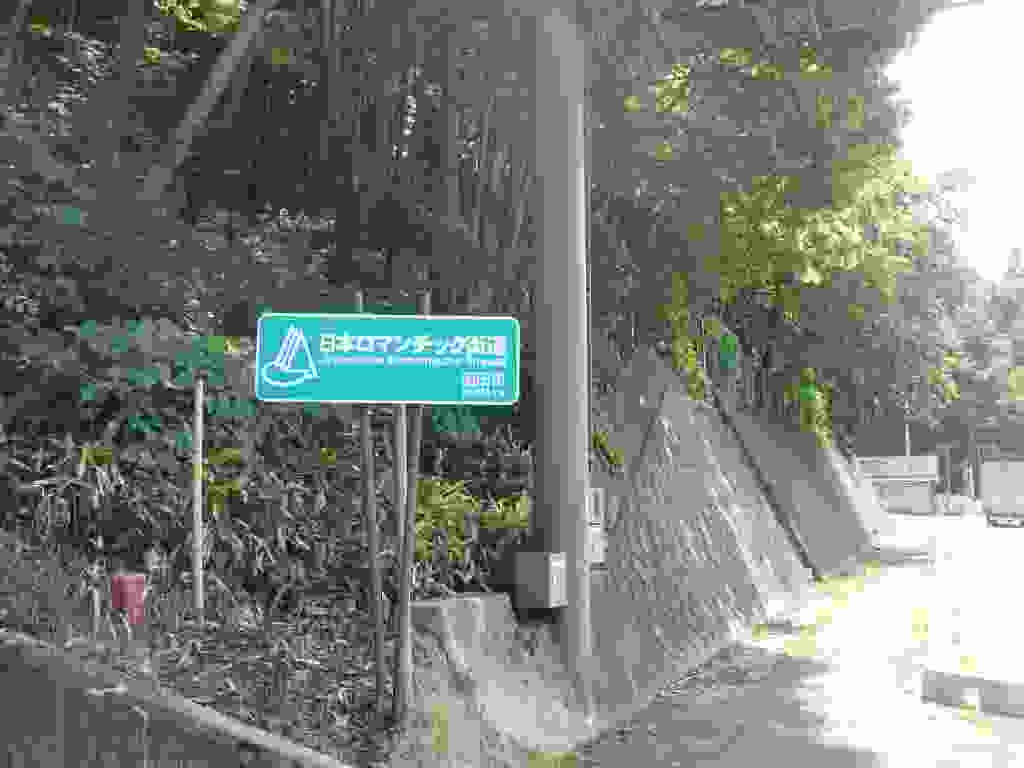
\includegraphics[width=\mywidth]{../wp-content/uploads/2015/08/P7315852-1024x768.jpg} \end{center}
\begin{center} 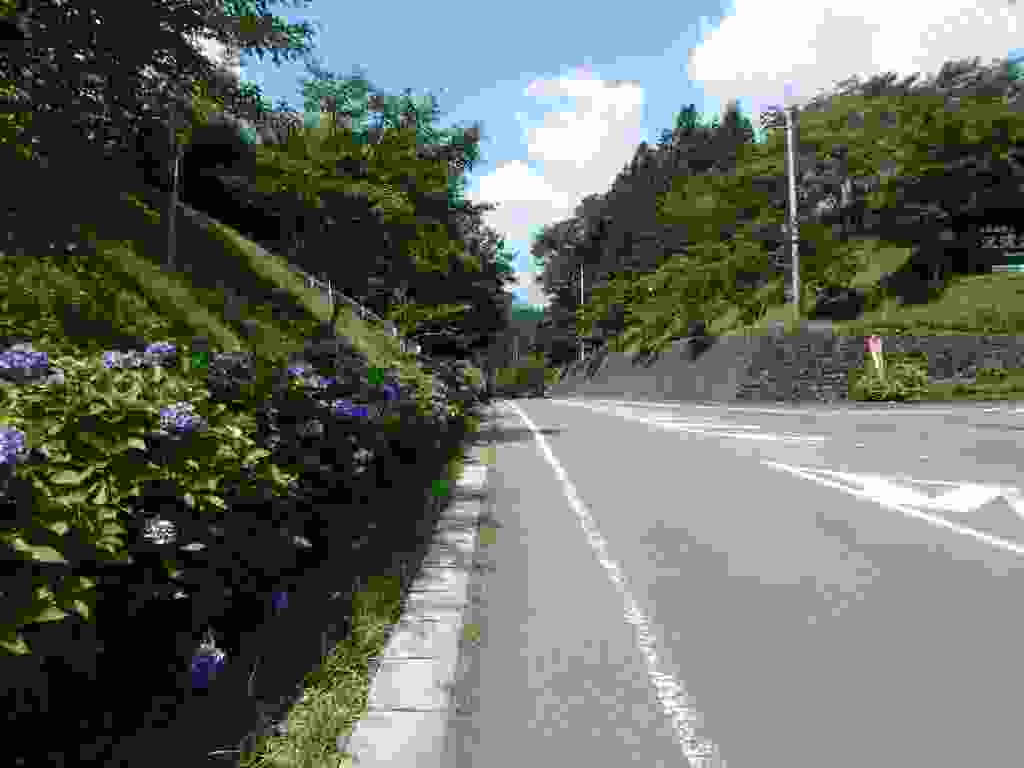
\includegraphics[width=\mywidth]{../wp-content/uploads/2015/08/P8015869-1024x768.jpg} \end{center}
\vspace{-\topsep}
\vspace{-2.75mm}
\pagebreak
~
\begin{center} 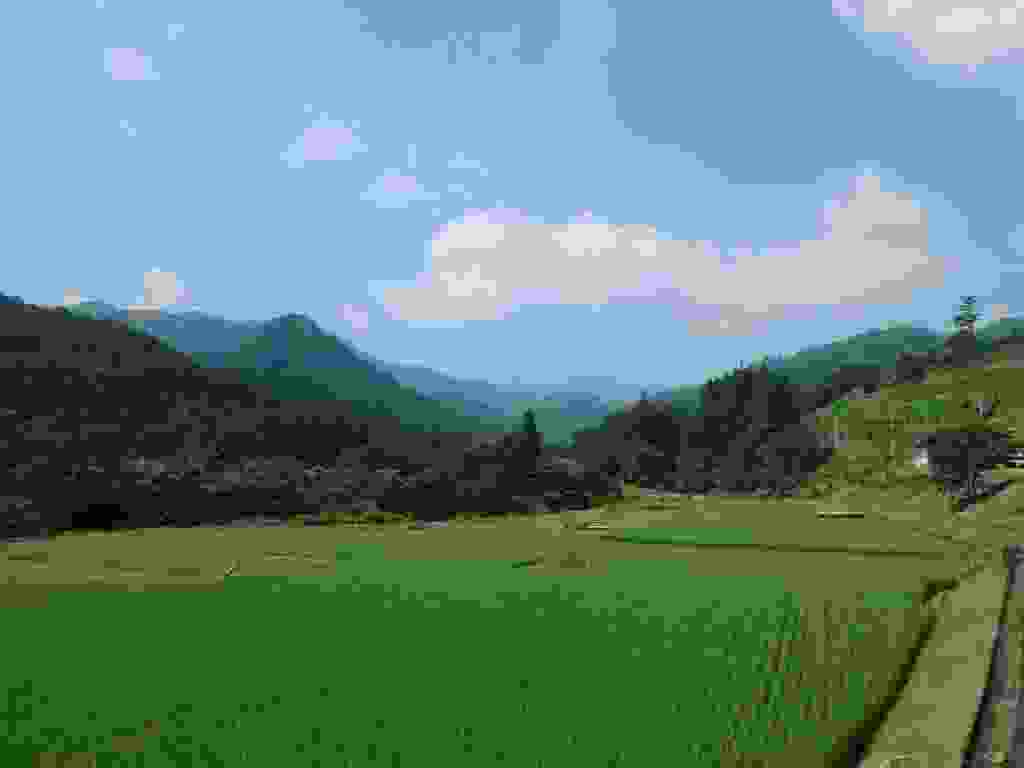
\includegraphics[width=\mywidth]{../wp-content/uploads/2015/08/P8015870-1024x768.jpg} \end{center}
\begin{center} 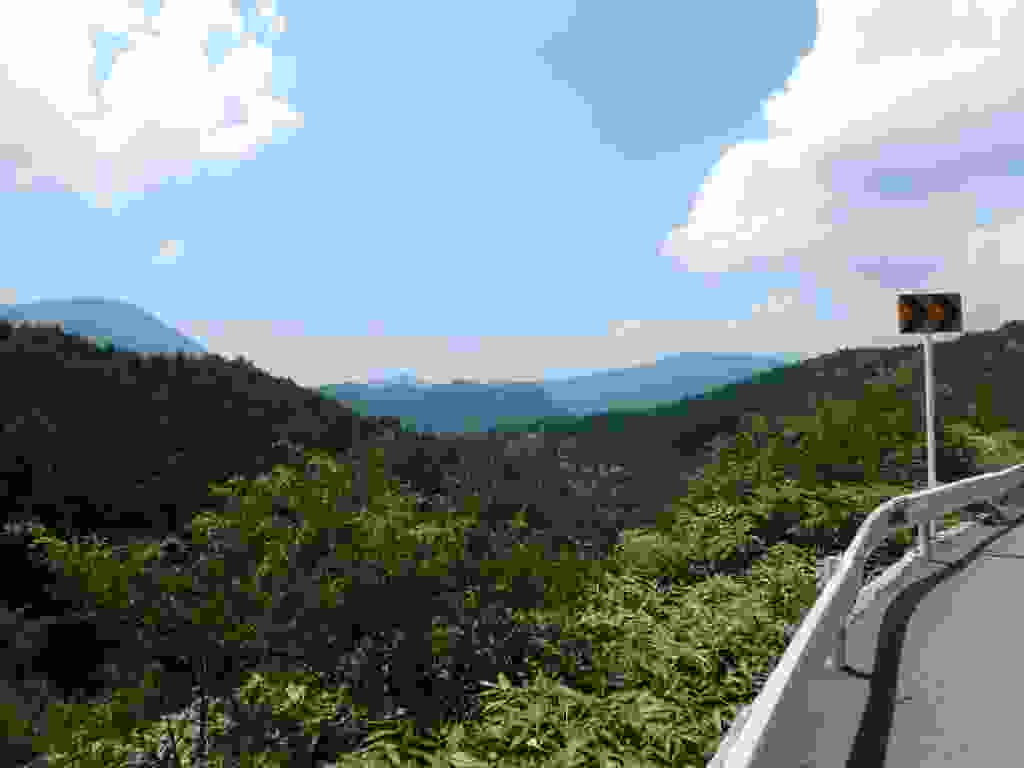
\includegraphics[width=\mywidth]{../wp-content/uploads/2015/08/P8025904-1024x768.jpg} \end{center}
\vspace{-\topsep}
\vspace{-3.25mm}
\pagebreak

 Pause pour aller voir la cascade de Fukiwari.
\begin{center} 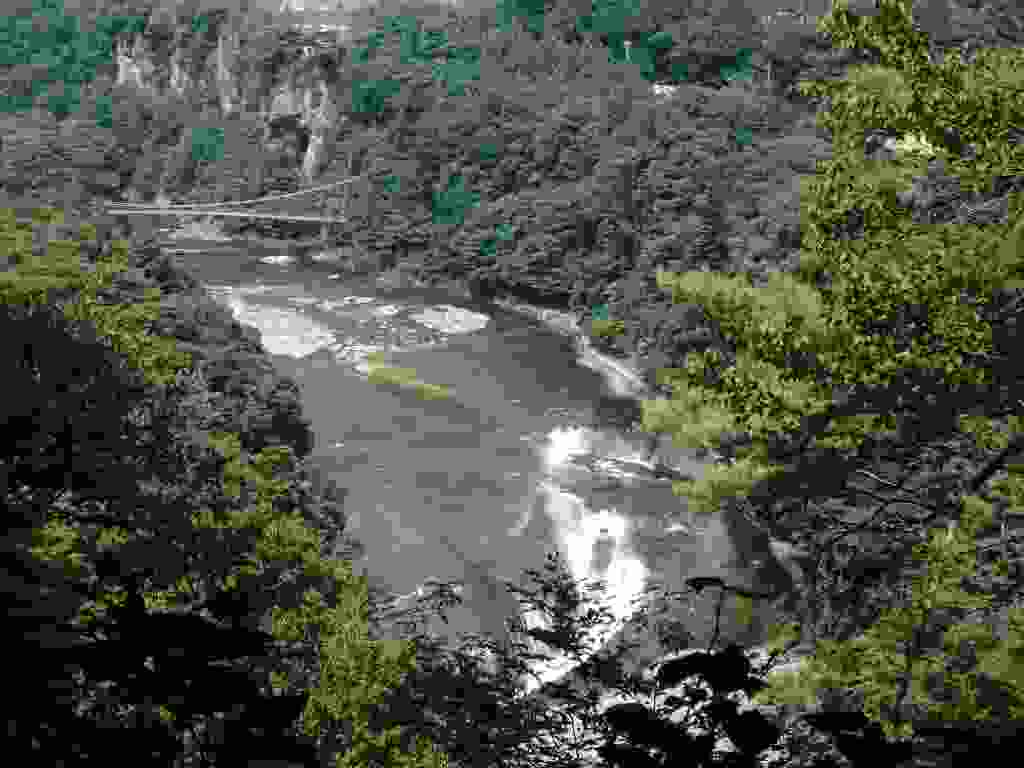
\includegraphics[width=\mywidth]{../wp-content/uploads/2015/08/P7315856-1024x768.jpg} \end{center}
\begin{center} 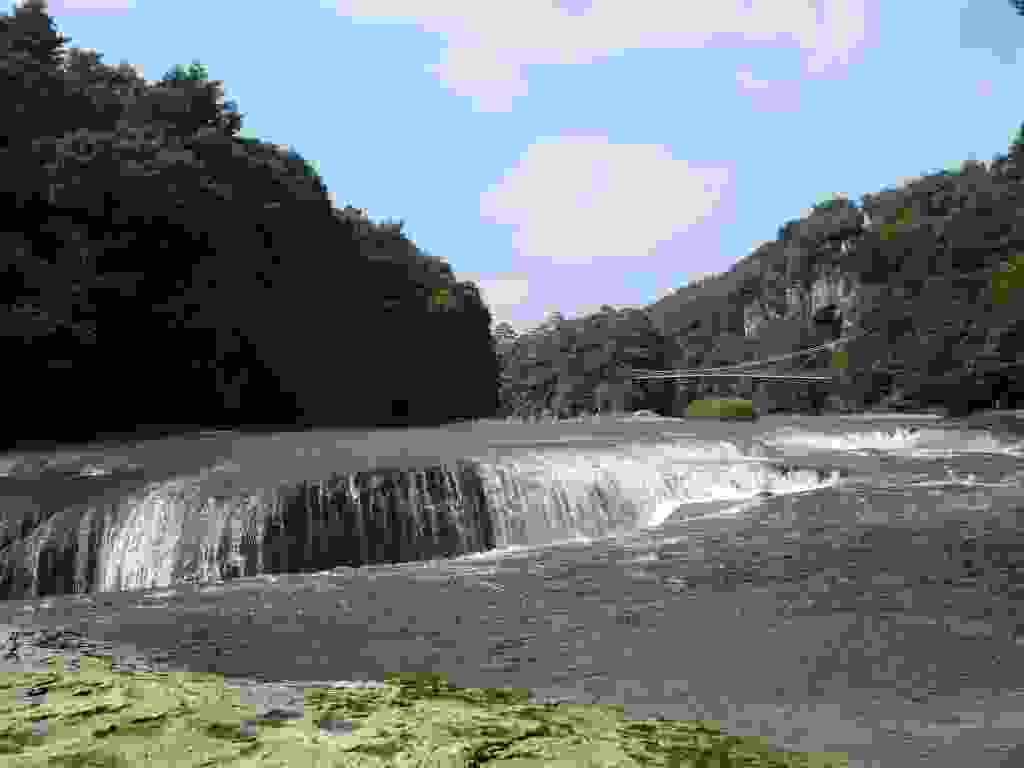
\includegraphics[width=\mywidth]{../wp-content/uploads/2015/08/P7315860-1024x768.jpg} \end{center}
\vspace{-\topsep}
\vspace{-3.25mm}
\pagebreak

 Je passe une soirée à Kusatsu, célèbre dans tout le Japon pour les vertus de son eau chaude naturelle. 
\begin{center} 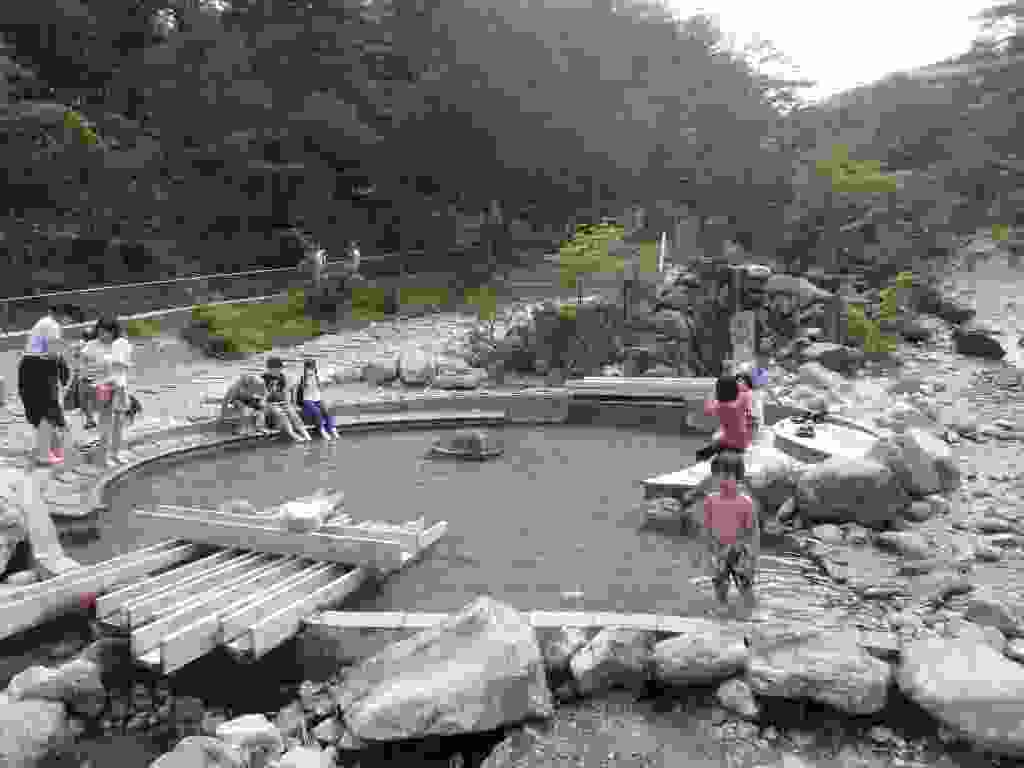
\includegraphics[width=\mywidth]{../wp-content/uploads/2015/08/P8015876-1024x768.jpg} \end{center}
\begin{center} 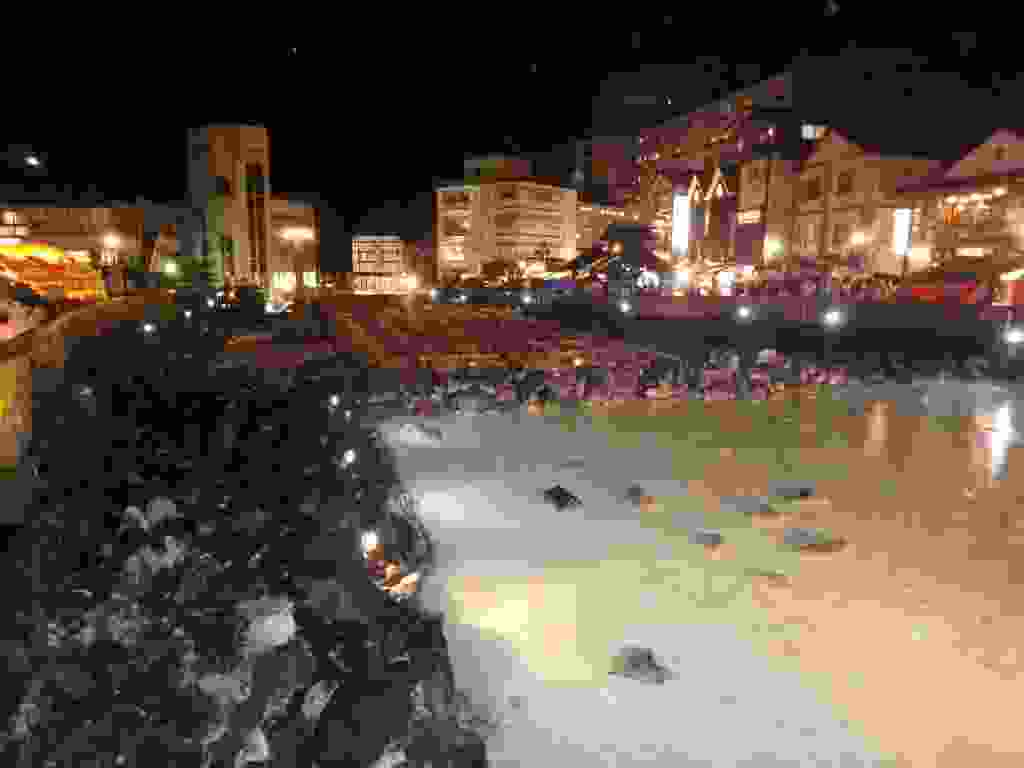
\includegraphics[width=\mywidth]{../wp-content/uploads/2015/08/P8015884-1024x768.jpg} \end{center}
\vspace{-\topsep}
\vspace{-2.75mm}
\pagebreak

 J'ai eu la chance d'y être le jour d'un festival, avec une représentation dédiée à l'eau.  
\begin{center} 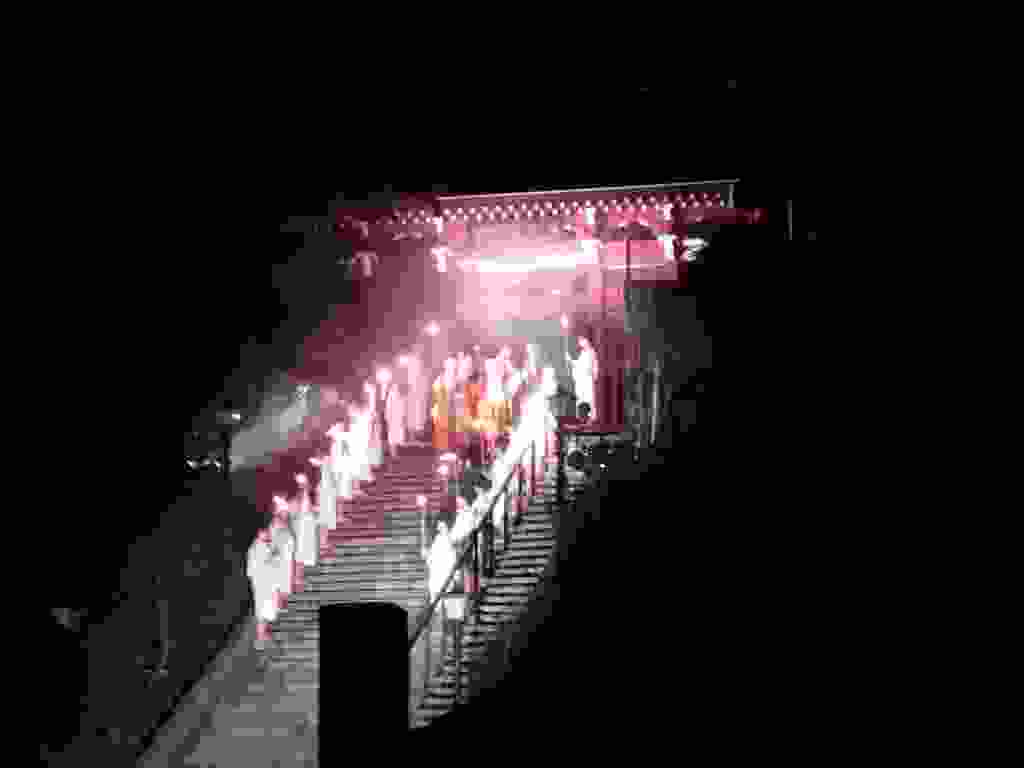
\includegraphics[width=\mywidth]{../wp-content/uploads/2015/08/P8015890-1024x768.jpg} \end{center}
\begin{center} 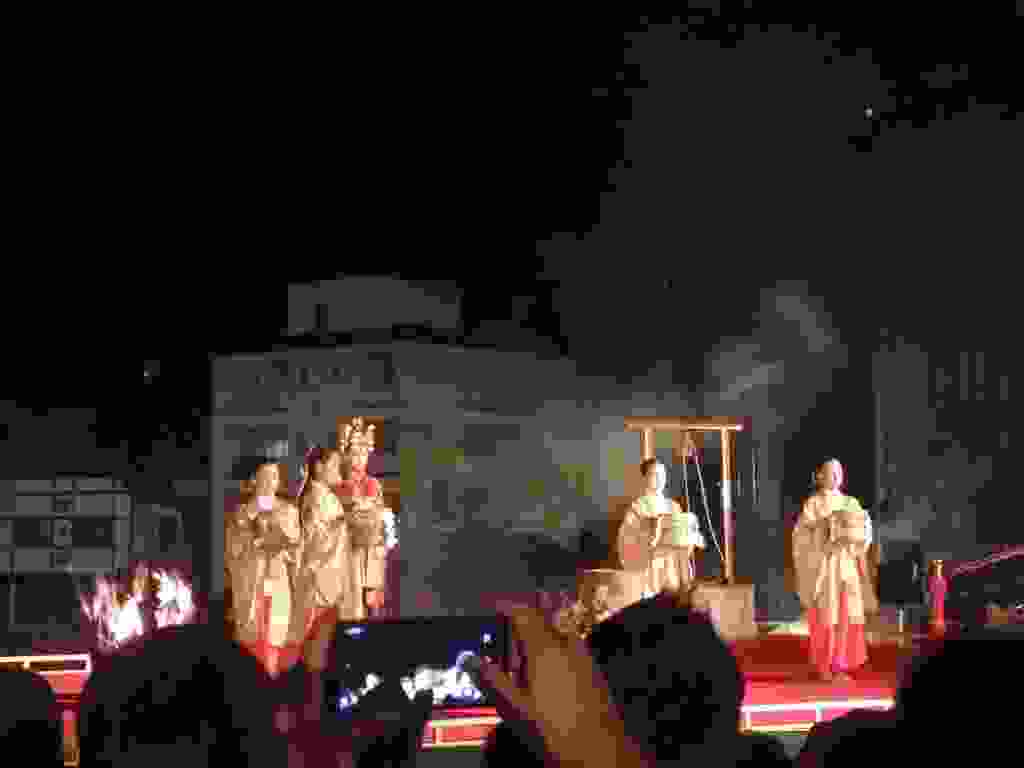
\includegraphics[width=\mywidth]{../wp-content/uploads/2015/08/P8015896-1024x768.jpg} \end{center}
\vspace{-\topsep}
\vspace{-2.75mm}
\pagebreak

 J'ai passé la nuit dans un hôtel, voici le petit déjeuner japonais.
\begin{center} 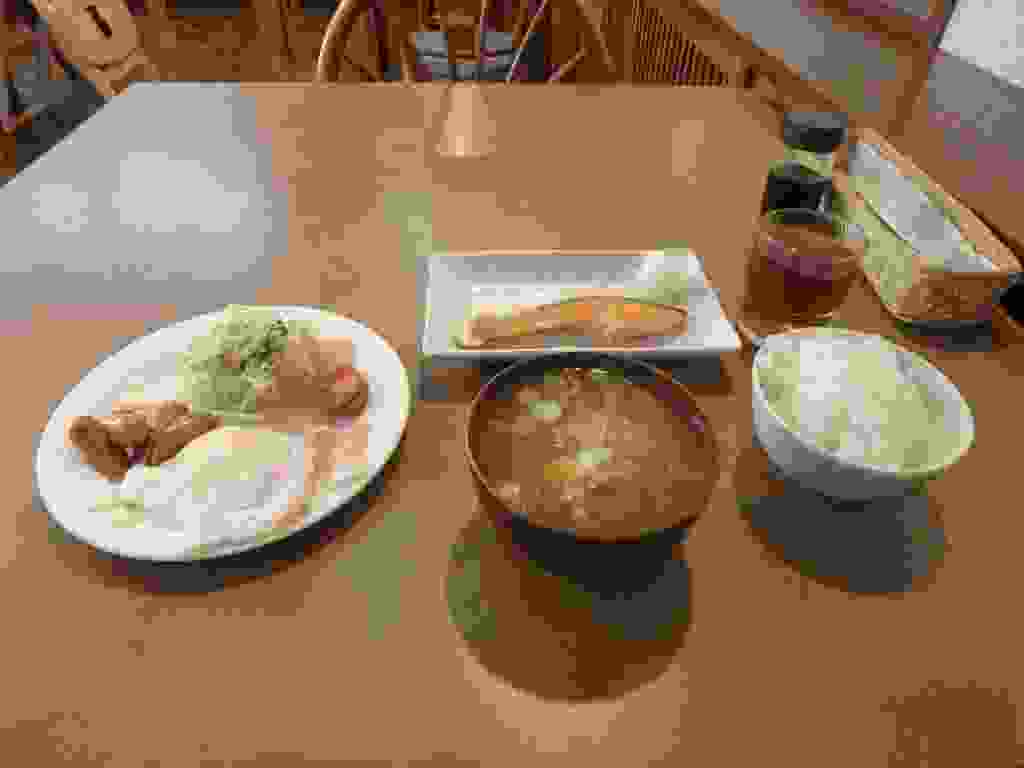
\includegraphics[width=\mywidth]{../wp-content/uploads/2015/08/P8025902-1024x768.jpg} \end{center}

 Enfin j'arrive à Nagano où je visite le temple de Zenkoji, construit tout en bois. 
\begin{center} \includegraphics[width=\mywidth]{../wp-content/uploads/2015/08/P8025915-1024x768.jpg} \end{center}
\vspace{-\topsep}
\pagebreak
~
\vspace{1mm}
\vfill
\begin{center} \includegraphics[width=\mywidth]{../wp-content/uploads/2015/08/P8025925-1024x768.jpg} \end{center}
\vfill
~\\
\vfill
\begin{center} \includegraphics[width=\mywidth]{../wp-content/uploads/2015/08/P8025919-1024x768.jpg} \end{center}
\vspace{-\topsep}
\vspace{-0.75mm}